% example.tex
% -----------------------------------------------------------------------------
% Worked example: decomposing a long-form paragraph into atomic units and
% inferring the relations between them.
%
% Two relation types are modeled:
%   * logical prerequisite   A -> B   (A must be true for B to be true/meaningful)
%   * position invalidation  A != B   (A, true at its position, contradicts a
%                                       claim B that appears later in the text)
%
% Compile with:  pdflatex example.tex   (run twice so TikZ positions settle)
% -----------------------------------------------------------------------------
\documentclass[11pt]{article}

\usepackage[margin=1in]{geometry}
\usepackage{amsmath}
\usepackage{enumitem}
\usepackage{xcolor}
\usepackage{soul}
\usepackage{tikz}
\usetikzlibrary{arrows.meta,positioning,calc,backgrounds}

% --- atomic-unit highlight palette (shared across all examples) ---
% Example 1 (damages) clusters; F9 is the pivot:
\definecolor{cBreach}{RGB}{210,228,248}   % breach cluster (F1--F4)
\definecolor{cArgue} {RGB}{252,243,207}    % defendant's argument (F5--F6)
\definecolor{cAgree} {RGB}{215,236,219}    % agreement / fraud (F7,F8,F10)
\definecolor{cPivot} {RGB}{250,219,180}    % pivot (void ab initio / revelation)
\definecolor{cUnjust}{RGB}{198,231,201}    % unjust enrichment (F11--F13)
% Example 2 (biography) topic groups:
\definecolor{cId}    {RGB}{210,228,248}   % identity / biographical
\definecolor{cCareer}{RGB}{252,243,207}    % career
\definecolor{cFilm}  {RGB}{215,236,219}    % film credits
\definecolor{cTV}    {RGB}{226,221,243}    % television credits
\definecolor{cStage} {RGB}{249,222,229}    % theater
\definecolor{cVoice} {RGB}{250,219,180}    % persona / voice
% contradiction roles (examples 2--5):
\definecolor{cEarly} {RGB}{198,231,201}    % earlier (asserted-first) atom
\definecolor{cLate}  {RGB}{248,205,205}    % later contradicting atom
% generic rotating palette (examples 3--5):
\definecolor{cP1}{RGB}{210,228,248}
\definecolor{cP2}{RGB}{252,243,207}
\definecolor{cP3}{RGB}{215,236,219}
\definecolor{cP4}{RGB}{226,221,243}
\definecolor{cP5}{RGB}{249,222,229}
\definecolor{cP6}{RGB}{222,240,243}
% legal-case roles (example 5):
\definecolor{cFact} {RGB}{210,228,248}   % neutral fact
\definecolor{cClaim}{RGB}{248,205,205}    % Renda's claim / position
\definecolor{cTruth}{RGB}{198,231,201}    % conceded truth
\definecolor{cHold} {RGB}{250,219,180}    % court's holding

% \fu{colour}{span}{label}: highlight a clause and tag it with its atomic-unit id.
% \hl (soul) wraps across line breaks; money amounts are kept in \mbox so the
% \$ does not trip soul's tokenizer.
\sethlcolor{cBreach}
\newcommand{\fu}[3]{{\sethlcolor{#1}\hl{#2}}\,\textsuperscript{\textbf{\scriptsize #3}}}

\title{Atomic-Unit Decomposition and Relation Inference\\\large A Worked Example}
\author{FactReasoner --- Ideation}
\date{\today}

\begin{document}
\maketitle

\section{Source paragraph}

\noindent\textbf{Plain text.}
\begin{quote}
The defendant was found liable for breach of contract, which occurred on
March 15, 2022, after they failed to deliver the specified goods. As a result,
the court awarded the plaintiff \$50,000 in damages for the breach. However, the
defendant argued that the plaintiff's own actions constituted a prior breach,
thus excusing their performance. The case hinged on the initial agreement signed
on January 1, 2022, which the court ultimately declared void ab initio (void from
the beginning) due to fraudulent misrepresentation by the plaintiff. Separately,
the court found the defendant liable for unjust enrichment and awarded the
plaintiff \$10,000 on that basis, as the defendant had retained a down payment.
\end{quote}

\noindent\textbf{Annotated.} Each highlighted clause is one atomic unit, tagged
with its identifier \textsuperscript{\textbf{\scriptsize F\textit{n}}}. Colours
group the units into the four clusters used later in the relation graph.

\begin{quote}
The defendant was \fu{cBreach}{found liable for breach of contract}{F1}, which
occurred \fu{cBreach}{on March 15, 2022}{F2}, after they
\fu{cBreach}{failed to deliver the specified goods}{F3}. As a result, the court
\fu{cBreach}{awarded the plaintiff \mbox{\$50,000} in damages for the breach}{F4}.
However, the defendant argued that
\fu{cArgue}{the plaintiff's own actions constituted a prior breach}{F5},
\fu{cArgue}{thus excusing their performance}{F6}.
\fu{cAgree}{The case hinged on the initial agreement}{F7}, signed
\fu{cAgree}{on January 1, 2022}{F8}, which the court ultimately
\fu{cPivot}{declared void ab initio (void from the beginning)}{F9} due to
\fu{cAgree}{fraudulent misrepresentation by the plaintiff}{F10}. Separately, the
court \fu{cUnjust}{found the defendant liable for unjust enrichment}{F11} and
\fu{cUnjust}{awarded the plaintiff \mbox{\$10,000} on that basis}{F12}, as the
\fu{cUnjust}{defendant had retained a down payment}{F13}.
\end{quote}

\noindent{\footnotesize\textbf{Legend:}~
\sethlcolor{cBreach}\hl{~breach of contract (F1--F4)~}\quad
\sethlcolor{cArgue}\hl{~defendant's argument (F5--F6)~}\quad
\sethlcolor{cPivot}\hl{~pivot: void ab initio (F9)~}\\[2pt]
\sethlcolor{cAgree}\hl{~agreement / fraud (F7, F8, F10)~}\quad
\sethlcolor{cUnjust}\hl{~unjust enrichment (F11--F13)~}\quad
The tag \textsuperscript{\textbf{\scriptsize F\textit{n}}} gives each unit's id.}

\section{Atomic units (in order of appearance)}

An \emph{atomic unit} is a short, self-contained sentence carrying exactly one
fact or claim.

\begin{enumerate}[label=\textbf{F\arabic*.},leftmargin=*]
  \item The defendant was found liable for breach of contract.
  \item The breach of contract occurred on March 15, 2022.
  \item The defendant failed to deliver the specified goods.
  \item The court awarded the plaintiff \$50,000 in damages for the breach.
  \item The defendant argued that the plaintiff's own actions constituted a prior breach.
  \item The defendant argued that the plaintiff's prior breach excused the defendant's performance.
  \item The case hinged on the initial agreement.
  \item The initial agreement was signed on January 1, 2022.
  \item The court declared the initial agreement void ab initio (void from the beginning).
  \item The agreement was declared void due to fraudulent misrepresentation by the plaintiff.
  \item The court found the defendant liable for unjust enrichment.
  \item The court awarded the plaintiff \$10,000 on the basis of unjust enrichment.
  \item The defendant had retained a down payment.
\end{enumerate}

\section{Relations}

\subsection*{Logical prerequisites ($A \rightarrow B$)}
\begin{itemize}[leftmargin=*]
  \item F3 $\rightarrow$ F1 --- failing to deliver the goods grounds the breach finding.
  \item F1 $\rightarrow$ F2 --- the breach must exist for it to have a date.
  \item F1 $\rightarrow$ F4 --- liability for breach is required to award damages ``for the breach.''
  \item F7 $\rightarrow$ F1 --- an initial agreement must exist for there to be a contract to breach.
  \item F7 $\rightarrow$ F8 --- the agreement must exist for it to have a signing date.
  \item F7 $\rightarrow$ F9 --- the agreement must exist for the court to declare it void.
  \item F8 $\rightarrow$ F9 --- the agreement signed Jan~1, 2022 is the thing declared void.
  \item F10 $\rightarrow$ F9 --- fraudulent misrepresentation is the stated cause of the voidness.
  \item F13 $\rightarrow$ F11 --- retaining the down payment grounds the unjust-enrichment finding.
  \item F11 $\rightarrow$ F12 --- the unjust-enrichment finding grounds the \$10,000 award.
\end{itemize}

\subsection*{Position invalidations ($A \neq B$)}
\begin{itemize}[leftmargin=*]
  \item F9 $\neq$ F1 --- void \emph{ab initio} means no valid contract ever existed,
        so the earlier breach-of-contract finding is invalidated.
  \item F9 $\neq$ F2 --- a breach ``on March 15, 2022'' cannot stand once no valid
        contract existed on that date.
  \item F9 $\neq$ F4 --- the \$50,000 damages award rests on a breach that is now
        deemed never to have occurred.
  \item F9 $\neq$ F6 --- there was no valid performance obligation to be ``excused.''
  \item F10 $\neq$ F5 --- the plaintiff's fraud supersedes the defendant's
        ``prior breach by plaintiff'' argument with a stronger ground.
\end{itemize}

\noindent
\textbf{Note.} The unjust-enrichment chain (F11, F12, F13), flagged
``Separately,'' is \emph{not} invalidated by F9: restitution for unjust
enrichment applies precisely \emph{because} no valid contract exists, so it is
consistent with --- even reinforced by --- the void declaration.

\section{Relation graph}

Solid blue arrows are logical prerequisites ($A \rightarrow B$). Dashed red
arrows are position invalidations ($A \neq B$). The pivotal unit \textbf{F9}
(void \emph{ab initio}) is highlighted: it retroactively invalidates the earlier
breach claims, while the unjust-enrichment cluster on the right survives.

\begin{center}
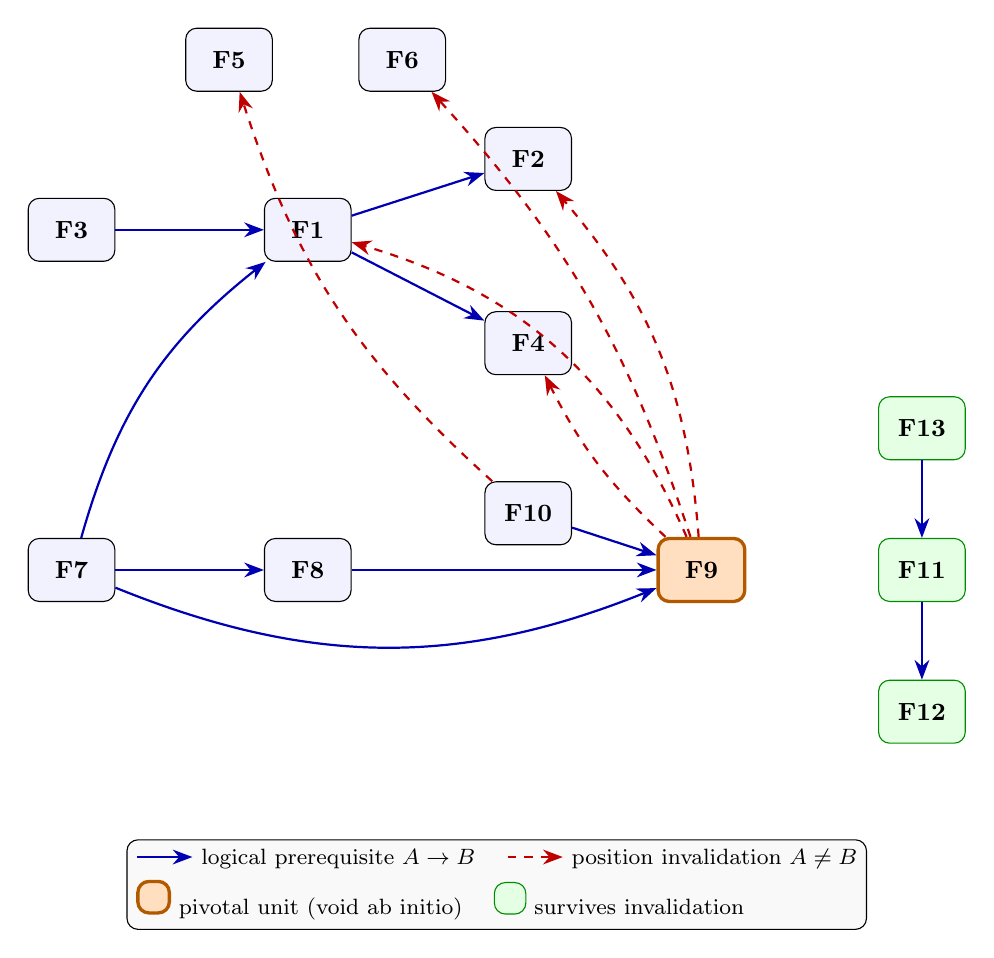
\begin{tikzpicture}[
    >={Stealth[length=2.5mm]},
    x=20mm, y=18mm,
    unit/.style={draw,rounded corners,minimum width=11mm,minimum height=8mm,
                 inner sep=1pt,font=\small\bfseries,fill=blue!5},
    pivot/.style={unit,fill=orange!25,draw=orange!70!black,very thick},
    survive/.style={unit,fill=green!10,draw=green!55!black},
    prereq/.style={->,blue!70!black,thick},
    invalid/.style={->,red!75!black,dashed,thick},
  ]

  % Nodes placed on an explicit (col,row) grid so none overlap.
  % Distinct columns: F2/F4 sit at col 2.9; F9/F10 at col 4.0; UE at col 5.4.
  % Distinct rows keep the F4 / F10 stack well separated.

  % --- defendant's argument (top row) ---
  \node[unit] (f5) at (1.0,3.6) {F5};
  \node[unit] (f6) at (2.1,3.6) {F6};

  % --- breach-of-contract cluster ---
  \node[unit] (f3) at (0,2.4)   {F3};
  \node[unit] (f1) at (1.5,2.4) {F1};
  \node[unit] (f2) at (2.9,2.9) {F2};
  \node[unit] (f4) at (2.9,1.6) {F4};

  % --- agreement / fraud cluster (bottom) ---
  \node[unit]  (f7)  at (0,0)    {F7};
  \node[unit]  (f8)  at (1.5,0)  {F8};
  \node[unit]  (f10) at (2.9,0.4) {F10};
  \node[pivot] (f9)  at (4.0,0)  {F9};

  % --- unjust-enrichment cluster (right, survives) ---
  \node[survive] (f13) at (5.4,1.0)  {F13};
  \node[survive] (f11) at (5.4,0)    {F11};
  \node[survive] (f12) at (5.4,-1.0) {F12};

  % --- logical prerequisites ---
  \draw[prereq] (f3) -- (f1);
  \draw[prereq] (f1) -- (f2);
  \draw[prereq] (f1) -- (f4);
  \draw[prereq] (f7) to[bend left=18] (f1);
  \draw[prereq] (f7) -- (f8);
  \draw[prereq] (f7) to[bend right=22] (f9);
  \draw[prereq] (f8) -- (f9);
  \draw[prereq] (f10) -- (f9);
  \draw[prereq] (f13) -- (f11);
  \draw[prereq] (f11) -- (f12);

  % --- position invalidations (from F9 / F10) ---
  \draw[invalid] (f9) to[bend right=25] (f1);
  \draw[invalid] (f9) to[bend right=18] (f2);
  \draw[invalid] (f9) to[bend left=10]  (f4);
  \draw[invalid] (f9) to[bend right=12] (f6);
  \draw[invalid] (f10) to[bend left=15] (f5);

  % --- legend (below the figure, full width) ---
  \node[draw,fill=gray!5,rounded corners,anchor=north,align=left,
        font=\footnotesize] at (2.7,-1.9) {
    \tikz\draw[prereq](0,0)--(7mm,0);~logical prerequisite $A\rightarrow B$
    \quad
    \tikz\draw[invalid](0,0)--(7mm,0);~position invalidation $A\neq B$\\[3pt]
    \tikz\node[pivot,minimum width=4mm,minimum height=4mm]{};~pivotal unit (void ab initio)
    \quad
    \tikz\node[survive,minimum width=4mm,minimum height=4mm]{};~survives invalidation
  };

\end{tikzpicture}
\end{center}

% =============================================================================
\section{Second example: a biography}

\subsection*{Source paragraph}

\noindent\textbf{Plain text.}
\begin{quote}
Lanny Flaherty is an American actor born on December 18, 1949, in Pensacola,
Florida. He has appeared in numerous films, television shows, and theater
productions throughout his career, which began in the late 1970s. Some of his
notable film credits include ``King of New York,'' ``The Abyss,'' ``Natural Born
Killers,'' ``The Game,'' and ``The Straight Story.'' On television, he has
appeared in shows such as ``Law \& Order,'' ``The Sopranos,'' ``Boardwalk
Empire,'' and ``The Leftovers.'' Flaherty has also worked extensively in theater,
including productions at the Public Theater and the New York Shakespeare
Festival. He is known for his distinctive looks and deep gravelly voice, which
have made him a memorable character actor in the industry.
\end{quote}

\noindent\textbf{Annotated.} Each highlighted clause is one atomic unit
\textsuperscript{\textbf{\scriptsize F\textit{n}}}; colours group units by topic
(identity, career, film, television, theater, persona).

\begin{quote}
\fu{cId}{Lanny Flaherty is an American actor}{F1} born
\fu{cId}{on December 18, 1949}{F2}, \fu{cId}{in Pensacola, Florida}{F3}.
\fu{cCareer}{He has appeared in numerous films, television shows, and theater productions}{F4}
throughout \fu{cCareer}{his career, which began in the late 1970s}{F5}. Some of
his notable film credits include \fu{cFilm}{``King of New York,''}{F6}
\fu{cFilm}{``The Abyss,''}{F7} \fu{cFilm}{``Natural Born Killers,''}{F8}
\fu{cFilm}{``The Game,''}{F9} and \fu{cFilm}{``The Straight Story.''}{F10} On
television, he has appeared in shows such as \fu{cTV}{``Law \& Order,''}{F11}
\fu{cTV}{``The Sopranos,''}{F12} \fu{cTV}{``Boardwalk Empire,''}{F13} and
\fu{cTV}{``The Leftovers.''}{F14} \fu{cStage}{Flaherty has also worked extensively in theater}{F15},
including productions at the \fu{cStage}{Public Theater}{F16} and the
\fu{cStage}{New York Shakespeare Festival}{F17}. He is known for his
\fu{cVoice}{distinctive looks and deep gravelly voice}{F18}, which
\fu{cVoice}{have made him a memorable character actor}{F19} in the industry.
\end{quote}

\subsection*{Atomic units (in order of appearance)}

\begin{enumerate}[label=\textbf{F\arabic*.},leftmargin=*]
  \item Lanny Flaherty is an American actor.
  \item Lanny Flaherty was born on December 18, 1949.
  \item Lanny Flaherty was born in Pensacola, Florida.
  \item Lanny Flaherty has appeared in numerous films, television shows, and theater productions.
  \item Lanny Flaherty's career began in the late 1970s.
  \item Lanny Flaherty's notable film credits include ``King of New York.''
  \item Lanny Flaherty's notable film credits include ``The Abyss.''
  \item Lanny Flaherty's notable film credits include ``Natural Born Killers.''
  \item Lanny Flaherty's notable film credits include ``The Game.''
  \item Lanny Flaherty's notable film credits include ``The Straight Story.''
  \item Lanny Flaherty has appeared in the television show ``Law \& Order.''
  \item Lanny Flaherty has appeared in the television show ``The Sopranos.''
  \item Lanny Flaherty has appeared in the television show ``Boardwalk Empire.''
  \item Lanny Flaherty has appeared in the television show ``The Leftovers.''
  \item Lanny Flaherty has worked extensively in theater.
  \item Lanny Flaherty's theater work includes productions at the Public Theater.
  \item Lanny Flaherty's theater work includes productions at the New York Shakespeare Festival.
  \item Lanny Flaherty is known for his distinctive looks and deep gravelly voice.
  \item Lanny Flaherty's distinctive looks and voice have made him a memorable character actor.
\end{enumerate}

\subsection*{Relations}

\textbf{Logical prerequisites ($A \rightarrow B$).} Here the prerequisite
relation is mostly one of \emph{subsumption / instantiation}: the general claim
that he appeared in films, TV, and theater (F4) underpins each specific credit,
and the identity claim (F1) underpins everything.

\begin{itemize}[leftmargin=*]
  \item F1 $\rightarrow$ F4 --- being an actor is presupposed by having a body of acting work.
  \item F1 $\rightarrow$ F5 --- being an actor is presupposed by having an acting career.
  \item F4 $\rightarrow$ F6,\,F7,\,F8,\,F9,\,F10 --- the general ``appeared in films'' claim subsumes each specific film credit.
  \item F4 $\rightarrow$ F11,\,F12,\,F13,\,F14 --- the general ``appeared in TV shows'' claim subsumes each specific show.
  \item F4 $\rightarrow$ F15 --- the general claim subsumes the theater-work claim.
  \item F15 $\rightarrow$ F16,\,F17 --- working in theater is presupposed by the specific theater venues.
  \item F18 $\rightarrow$ F19 --- the distinctive looks/voice are the stated cause of his being a memorable character actor.
  \item F1 $\rightarrow$ F19 --- being an actor is presupposed by being a memorable \emph{character} actor.
\end{itemize}

\noindent
\textbf{Position invalidations ($A \neq B$).} \emph{None.} Unlike the legal
example, this biography is monotonic: every later claim is consistent with the
earlier ones, and no statement retracts or contradicts a prior position. The
absence of invalidation edges is itself the finding.

\subsection*{Relation graph}

All edges are logical prerequisites / subsumption ($A \rightarrow B$); there are
no invalidation edges. The identity node \textbf{F1} is the root; the
``body of work'' node \textbf{F4} fans out to the specific credits.

\begin{center}
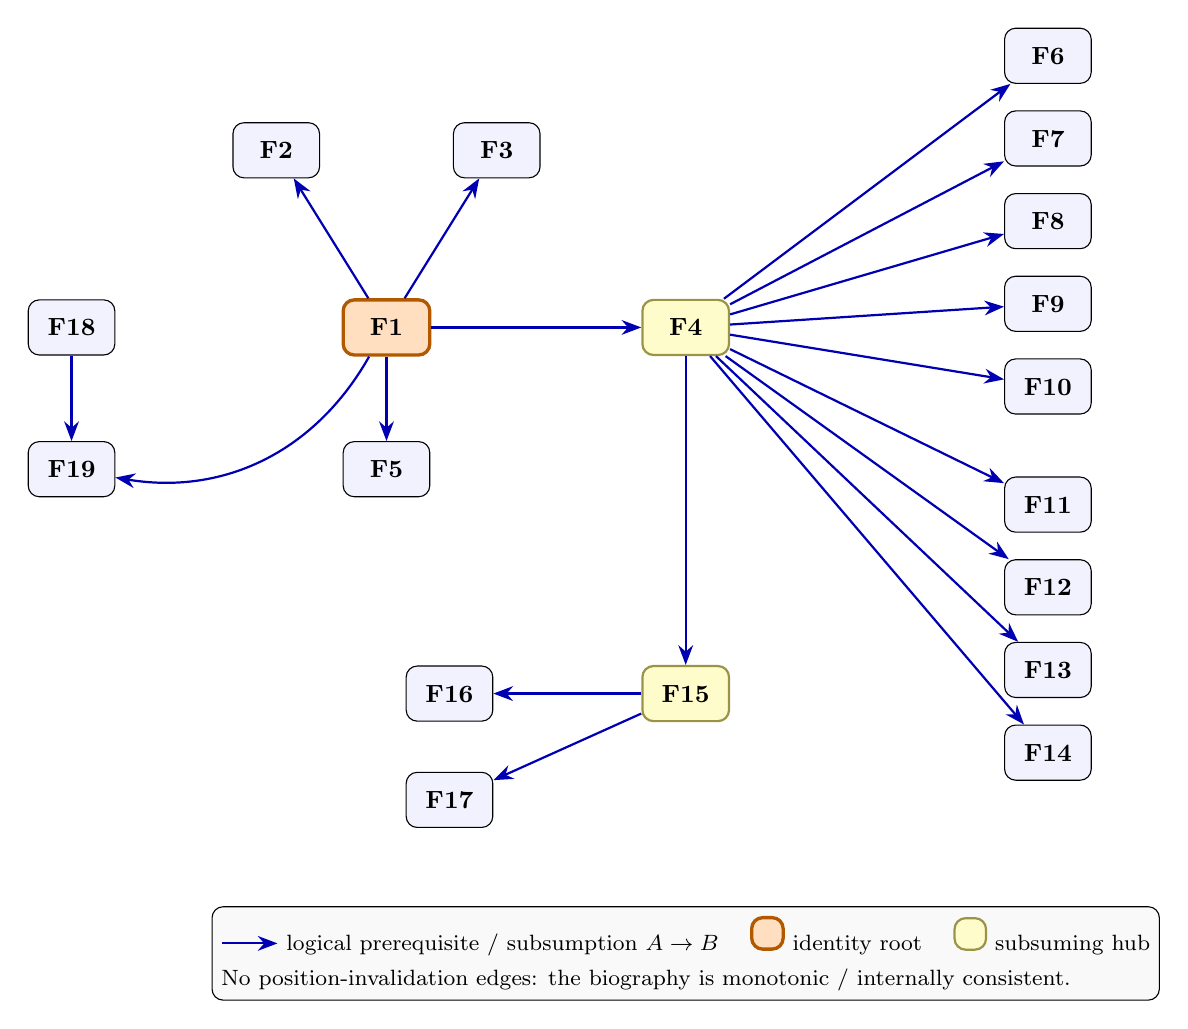
\begin{tikzpicture}[
    >={Stealth[length=2.5mm]},
    x=20mm, y=15mm,
    bnode/.style={draw,rounded corners,minimum width=11mm,minimum height=7mm,
                  inner sep=1pt,font=\small\bfseries,fill=blue!5},
    root/.style={bnode,fill=orange!25,draw=orange!70!black,very thick},
    hub/.style={bnode,fill=yellow!20,draw=yellow!55!black,thick},
    prereq/.style={->,blue!70!black,thick},
  ]

  % Explicit grid; generous spacing keeps every node clear of its neighbours
  % and of the edges. Films and TV are split into two separate columns so the
  % F4 fan-out never crowds a single tall stack.

  % --- persona (far left) ---
  \node[bnode] (f18) at (-2.0,1.7) {F18};
  \node[bnode] (f19) at (-2.0,0.5) {F19};

  % --- biographical facts (top, above the root) ---
  \node[bnode] (f2) at (-0.7,3.2) {F2};
  \node[bnode] (f3) at (0.7,3.2)  {F3};

  % --- root identity ---
  \node[root]  (f1) at (0,1.7) {F1};
  \node[bnode] (f5) at (0,0.5) {F5};

  % --- central "body of work" hub ---
  \node[hub] (f4) at (1.9,1.7) {F4};

  % --- film credits (right column, fanned upward) ---
  \node[bnode] (f6)  at (4.2,4.0) {F6};
  \node[bnode] (f7)  at (4.2,3.3) {F7};
  \node[bnode] (f8)  at (4.2,2.6) {F8};
  \node[bnode] (f9)  at (4.2,1.9) {F9};
  \node[bnode] (f10) at (4.2,1.2) {F10};

  % --- TV credits (right column, fanned downward; same column as films but
  %     a clear vertical gap below F10 so the fan never crosses a film node) ---
  \node[bnode] (f11) at (4.2,0.2)  {F11};
  \node[bnode] (f12) at (4.2,-0.5) {F12};
  \node[bnode] (f13) at (4.2,-1.2) {F13};
  \node[bnode] (f14) at (4.2,-1.9) {F14};

  % --- theater (below the hub, own column to the left of the credits) ---
  \node[hub]   (f15) at (1.9,-1.4) {F15};
  \node[bnode] (f16) at (0.4,-1.4) {F16};
  \node[bnode] (f17) at (0.4,-2.3) {F17};

  % --- edges from identity ---
  \draw[prereq] (f1) -- (f2);
  \draw[prereq] (f1) -- (f3);
  \draw[prereq] (f1) -- (f4);
  \draw[prereq] (f1) -- (f5);
  \draw[prereq] (f1) to[bend left=35] (f19);   % routed out to the left, clear of F18

  % --- F4 subsumes specific film credits ---
  \foreach \t in {f6,f7,f8,f9,f10} { \draw[prereq] (f4) -- (\t); }

  % --- F4 subsumes specific TV credits ---
  \foreach \t in {f11,f12,f13,f14} { \draw[prereq] (f4) -- (\t); }

  % --- F4 subsumes theater work, which subsumes the venues ---
  \draw[prereq] (f4) -- (f15);
  \draw[prereq] (f15) -- (f16);
  \draw[prereq] (f15) -- (f17);

  % --- persona cause ---
  \draw[prereq] (f18) -- (f19);

  % --- legend ---
  \node[draw,fill=gray!5,rounded corners,anchor=north,align=left,
        font=\footnotesize] at (1.9,-3.2) {
    \tikz\draw[prereq](0,0)--(7mm,0);~logical prerequisite / subsumption $A\rightarrow B$
    \quad
    \tikz\node[root,minimum width=4mm,minimum height=4mm]{};~identity root
    \quad
    \tikz\node[hub,minimum width=4mm,minimum height=4mm]{};~subsuming hub\\[3pt]
    No position-invalidation edges: the biography is monotonic / internally consistent.
  };

\end{tikzpicture}
\end{center}

\subsection*{A modified biography with planted contradictions}

The biography above is internally consistent, so it has no invalidation edges.
To illustrate the contradiction relation we now \emph{alter} the passage,
inserting later statements that conflict with earlier ones (different birth year
and place, a different nationality, a different career-start decade, and a voice
description that reverses the earlier one). Each contradiction is a positional
invalidation: the earlier atom, asserted first, is contradicted by a later atom.

\paragraph{Modified source paragraph (contradictions in \emph{italics}).}

\noindent\textbf{Plain text.}
\begin{quote}
Lanny Flaherty is an American actor born on December 18, 1949, in Pensacola,
Florida. His career began in the late 1970s, and he appeared in numerous films,
television shows, and theater productions. He is known for his deep gravelly
voice. \emph{Born in 1942, Flaherty was a Mississippi native who first appeared
on screen only in the 1990s.} Critics often described \emph{the British
character actor} for \emph{his soft, high-pitched voice}, which made him
instantly recognizable.
\end{quote}

\noindent\textbf{Annotated.} Each clause is one atomic unit
\textsuperscript{\textbf{\scriptsize M\textit{n}}}. Green marks an
earlier (asserted-first) atom and red the later atom that contradicts it; neutral
(blue) atoms are uncontested.

\begin{quote}
\fu{cEarly}{Lanny Flaherty is an American actor}{M1} born
\fu{cEarly}{on December 18, 1949}{M2}, \fu{cEarly}{in Pensacola, Florida}{M3}.
\fu{cEarly}{His career began in the late 1970s}{M4}, and
\fu{cId}{he appeared in numerous films, television shows, and theater productions}{M5}.
\fu{cEarly}{He is known for his deep gravelly voice}{M6}.
\emph{\fu{cLate}{Born in 1942}{M7}, \fu{cLate}{Flaherty was a Mississippi native}{M8}
\fu{cLate}{who first appeared on screen only in the 1990s}{M9}.} Critics often
described \emph{\fu{cLate}{the British character actor}{M10}} for
\emph{\fu{cLate}{his soft, high-pitched voice}{M11}}, which
\fu{cId}{made him instantly recognizable}{M12}.
\end{quote}

\paragraph{Atomic units (self-contained, in order of appearance).}
\begin{enumerate}[label=\textbf{M\arabic*.},leftmargin=*]
  \item Lanny Flaherty is an American actor.
  \item Lanny Flaherty was born on December 18, 1949.
  \item Lanny Flaherty was born in Pensacola, Florida.
  \item Lanny Flaherty's career began in the late 1970s.
  \item Lanny Flaherty appeared in numerous films, television shows, and theater productions.
  \item Lanny Flaherty is known for his deep gravelly voice.
  \item Lanny Flaherty was born in 1942.
  \item Lanny Flaherty was a Mississippi native.
  \item Lanny Flaherty first appeared on screen only in the 1990s.
  \item Lanny Flaherty is a British character actor.
  \item Lanny Flaherty has a soft, high-pitched voice.
  \item Lanny Flaherty's voice made him instantly recognizable.
\end{enumerate}

\subsubsection*{Relations}

\textbf{Logical prerequisites ($A \rightarrow B$).}
\begin{itemize}[leftmargin=*]
  \item M1 $\rightarrow$ M5 --- being an actor is presupposed by having a body of acting work.
  \item M1 $\rightarrow$ M4 --- being an actor is presupposed by having an acting career.
  \item M11 $\rightarrow$ M12 --- having a (distinctive) voice is presupposed by that voice making him recognizable.
\end{itemize}

\noindent
\textbf{Position invalidations ($A \neq B$).} Each later atom contradicts an
earlier one asserted at a different position.
\begin{itemize}[leftmargin=*]
  \item M2 $\neq$ M7 --- born December 18, 1949 contradicts born in 1942.
  \item M3 $\neq$ M8 --- born in Pensacola, Florida contradicts being a Mississippi native.
  \item M4 $\neq$ M9 --- a career beginning in the late 1970s contradicts first appearing on screen only in the 1990s.
  \item M1 $\neq$ M10 --- being an \emph{American} actor contradicts being a \emph{British} character actor.
  \item M6 $\neq$ M11 --- a deep gravelly voice contradicts a soft, high-pitched voice.
\end{itemize}

\noindent
\textbf{Note.} The contradictions are pairwise and local: each invalidation links
exactly one early biographical claim to its later mutually exclusive restatement.
The prerequisite structure (identity $\to$ work / career, voice $\to$
recognizability) is unaffected; M5 has no specific-credit children here because
the modified paragraph drops the individual titles.

\paragraph{Relation graph.}
Solid blue arrows are logical prerequisites ($A \rightarrow B$). Dashed red
arrows are position invalidations ($A \neq B$): each links an earlier
(\emph{green, asserted-first}) atom to the later (\emph{red}) atom that
contradicts it. The five contradiction pairs are stacked so no arrow crosses a
node.

\begin{center}
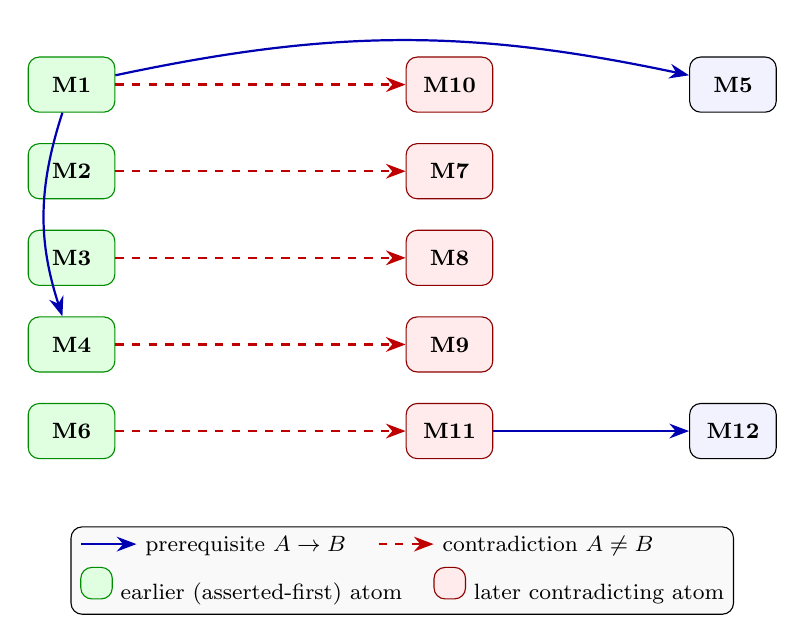
\begin{tikzpicture}[
    >={Stealth[length=2.5mm]},
    x=20mm, y=11mm,
    mnode/.style={draw,rounded corners,minimum width=11mm,minimum height=7mm,
                  inner sep=1pt,font=\footnotesize\bfseries,fill=blue!5},
    early/.style={mnode,fill=green!12,draw=green!55!black},
    late/.style={mnode,fill=red!8,draw=red!55!black},
    prereq/.style={->,blue!70!black,thick},
    invalid/.style={->,red!75!black,dashed,thick},
  ]

  % Left column: earlier (asserted-first) atoms. Right column: the later atoms
  % that contradict them. Each contradiction pair sits on its own row, so the
  % dashed edges are short horizontals that never cross a node.
  \node[early] (m1) at (0,4) {M1};
  \node[early] (m2) at (0,3) {M2};
  \node[early] (m3) at (0,2) {M3};
  \node[early] (m4) at (0,1) {M4};
  \node[early] (m6) at (0,0) {M6};

  \node[late] (m10) at (2.4,4) {M10};
  \node[late] (m7)  at (2.4,3) {M7};
  \node[late] (m8)  at (2.4,2) {M8};
  \node[late] (m9)  at (2.4,1) {M9};
  \node[late] (m11) at (2.4,0) {M11};

  % prerequisite-only atoms (right side, kept clear of the contradiction fan)
  \node[mnode] (m5)  at (4.2,4) {M5};
  \node[mnode] (m12) at (4.2,0) {M12};

  % --- contradiction edges (one per row) ---
  \draw[invalid] (m1) -- (m10);
  \draw[invalid] (m2) -- (m7);
  \draw[invalid] (m3) -- (m8);
  \draw[invalid] (m4) -- (m9);
  \draw[invalid] (m6) -- (m11);

  % --- prerequisite edges ---
  \draw[prereq] (m1) to[bend left=12] (m5);   % identity -> body of work
  \draw[prereq] (m1) to[bend right=18] (m4);   % identity -> career
  \draw[prereq] (m11) -- (m12);                % voice -> recognizable

  % --- legend ---
  \node[draw,fill=gray!5,rounded corners,anchor=north,align=left,
        font=\footnotesize] at (2.1,-1.1) {
    \tikz\draw[prereq](0,0)--(7mm,0);~prerequisite $A\rightarrow B$
    \quad
    \tikz\draw[invalid](0,0)--(7mm,0);~contradiction $A\neq B$\\[3pt]
    \tikz\node[early,minimum width=4mm,minimum height=4mm]{};~earlier (asserted-first) atom
    \quad
    \tikz\node[late,minimum width=4mm,minimum height=4mm]{};~later contradicting atom
  };

\end{tikzpicture}
\end{center}

% =============================================================================
\section{Third example: a narrative passage}

\subsection*{Source paragraph}

\noindent\textbf{Plain text.}
\begin{quote}
Elinor is surprised no letter arrives with details about the marriage, and she
wonders how Edward felt being close to Barton. Elinor asks her mother to write to
Colonel Brandon for news, realizing she hoped something would prevent Edward's
marriage. Elinor feels incredibly hurt by Edward's marriage. Colonel Brandon
arrives at the house, but it is revealed to be Edward instead. Elinor is surprised
that Edward and Lucy were married so soon, and she mulls over the event of
Edward's marriage, supposing that the Ferrars must be settled at Delaford,
envisioning Edward and Lucy's life there. Edward enters the room looking ill with
anxiety, and Elinor tells herself to be calm upon Edward's arrival. Elinor thinks
someone in London might have informed her about Edward and Lucy's marriage.
Marianne and Margaret retreat, leaving Elinor and Mrs.~Dashwood with Edward,
while Marianne and Mrs.~Dashwood react with shock and uncertainty about Edward's
arrival. Mrs.~Dashwood breaks the ice by shaking Edward's hand and wishing him
happiness. However, no word has arrived from Colonel Brandon, and Mrs.~Dashwood
asks about Mrs.~Ferrars' health, to which Elinor inquires if Mrs.~Ferrars is at
Longstaple. Edward is shocked to discover his mother is not nearby, and Elinor
pointedly asks about Mrs.~Edward Ferrars. Edward is confused and asks if Elinor
means Mrs.~Robert Ferrars instead, leading to everyone being shocked by the
revelation that Robert married Lucy Steele. Elinor flees the room, unsure of how
to react, and bursts into tears of joy. Edward sits in silence, unsure of what to
do, then simply leaves the room. Everyone is left perplexed by the situation.
\end{quote}

\noindent\textbf{Annotated.} Each highlighted clause is one atomic unit
\textsuperscript{\textbf{\scriptsize F\textit{n}}}; the rotating colours just
separate adjacent units, and the pivotal revelation \textbf{F27} is orange.

\begin{quote}
\fu{cP1}{Elinor is surprised no letter arrives with details about the marriage}{F1}, and she
\fu{cP2}{wonders how Edward felt being close to Barton}{F2}.
\fu{cP3}{Elinor asks her mother to write to Colonel Brandon for news}{F3},
\fu{cP4}{realizing she hoped something would prevent Edward's marriage}{F4}.
\fu{cP5}{Elinor feels incredibly hurt by Edward's marriage}{F5}.
\fu{cP6}{Colonel Brandon arrives at the house}{F6}, but
\fu{cP1}{it is revealed to be Edward instead}{F7}.
\fu{cP2}{Elinor is surprised that Edward and Lucy were married so soon}{F8}, and she
\fu{cP3}{mulls over the event of Edward's marriage}{F9},
\fu{cP4}{supposing that the Ferrars must be settled at Delaford}{F10},
\fu{cP5}{envisioning Edward and Lucy's life there}{F11}.
\fu{cP6}{Edward enters the room looking ill with anxiety}{F12}, and
\fu{cP1}{Elinor tells herself to be calm upon Edward's arrival}{F13}.
\fu{cP2}{Elinor thinks someone in London might have informed her about Edward and Lucy's marriage}{F14}.
\fu{cP3}{Marianne and Margaret retreat}{F15},
\fu{cP4}{leaving Elinor and Mrs.~Dashwood with Edward}{F16}, while
\fu{cP5}{Marianne and Mrs.~Dashwood react with shock and uncertainty about Edward's arrival}{F17}.
\fu{cP6}{Mrs.~Dashwood breaks the ice by shaking Edward's hand}{F18} and
\fu{cP1}{wishing him happiness}{F19}. However,
\fu{cP2}{no word has arrived from Colonel Brandon}{F20}, and
\fu{cP3}{Mrs.~Dashwood asks about Mrs.~Ferrars' health}{F21}, to which
\fu{cP4}{Elinor inquires if Mrs.~Ferrars is at Longstaple}{F22}.
\fu{cP5}{Edward is shocked to discover his mother is not nearby}{F23}, and
\fu{cP6}{Elinor pointedly asks about Mrs.~Edward Ferrars}{F24}.
\fu{cP1}{Edward is confused}{F25} and
\fu{cP2}{asks if Elinor means Mrs.~Robert Ferrars instead}{F26}, leading to
\fu{cP3}{everyone being shocked}{F28} by the
\fu{cPivot}{revelation that Robert married Lucy Steele}{F27}.
\fu{cP5}{Elinor flees the room, unsure of how to react}{F29}, and
\fu{cP6}{bursts into tears of joy}{F30}.
\fu{cP1}{Edward sits in silence, unsure of what to do}{F31},
\fu{cP2}{then simply leaves the room}{F32}.
\fu{cP3}{Everyone is left perplexed by the situation}{F33}.
\end{quote}

\subsection*{Atomic units (self-contained, in order of appearance)}

Pronouns are resolved to their referents so each unit stands alone.

\begin{enumerate}[label=\textbf{F\arabic*.},leftmargin=*]
  \item Elinor is surprised that no letter arrives with details about the marriage.
  \item Elinor wonders how Edward felt being close to Barton.
  \item Elinor asks her mother to write to Colonel Brandon for news.
  \item Elinor realizes she had hoped something would prevent Edward's marriage.
  \item Elinor feels incredibly hurt by Edward's marriage.
  \item A visitor arrives at the house and is initially taken to be Colonel Brandon.
  \item The visitor is revealed to be Edward instead of Colonel Brandon.
  \item Elinor is surprised that Edward and Lucy were married so soon.
  \item Elinor mulls over the event of Edward's marriage.
  \item Elinor supposes that the Ferrars must be settled at Delaford.
  \item Elinor envisions Edward and Lucy's life at Delaford.
  \item Edward enters the room looking ill with anxiety.
  \item Elinor tells herself to be calm upon Edward's arrival.
  \item Elinor thinks someone in London might have informed her about Edward and Lucy's marriage.
  \item Marianne and Margaret retreat from the room.
  \item Marianne and Margaret leave Elinor and Mrs.~Dashwood alone with Edward.
  \item Marianne and Mrs.~Dashwood react with shock and uncertainty about Edward's arrival.
  \item Mrs.~Dashwood breaks the ice by shaking Edward's hand.
  \item Mrs.~Dashwood wishes Edward happiness.
  \item No word has arrived from Colonel Brandon.
  \item Mrs.~Dashwood asks about Mrs.~Ferrars' health.
  \item Elinor inquires whether Mrs.~Ferrars is at Longstaple.
  \item Edward is shocked to discover Edward's mother is not nearby.
  \item Elinor pointedly asks about Mrs.~Edward Ferrars.
  \item Edward is confused by Elinor's question about Mrs.~Edward Ferrars.
  \item Edward asks whether Elinor means Mrs.~Robert Ferrars instead.
  \item It is revealed that Robert married Lucy Steele.
  \item Everyone is shocked by the revelation that Robert married Lucy Steele.
  \item Elinor flees the room, unsure of how to react.
  \item Elinor bursts into tears of joy.
  \item Edward sits in silence, unsure of what to do.
  \item Edward then leaves the room.
  \item Everyone is left perplexed by the situation.
\end{enumerate}

\subsection*{Relations}

\textbf{Logical prerequisites ($A \rightarrow B$).} In a narrative the
prerequisite relation is largely \emph{enabling causation / temporal grounding}:
an earlier event makes a later one possible or meaningful.

\begin{itemize}[leftmargin=*]
  \item F6 $\rightarrow$ F7 --- a visitor must arrive before being re-identified as Edward.
  \item F7 $\rightarrow$ F12 --- Edward being the arrival is presupposed by Edward entering the room.
  \item F9 $\rightarrow$ F10 --- mulling over the marriage grounds the supposition about Delaford.
  \item F10 $\rightarrow$ F11 --- supposing the Ferrars settle at Delaford grounds envisioning their life there.
  \item F15 $\rightarrow$ F16 --- Marianne and Margaret must retreat for Elinor and Mrs.~Dashwood to be left with Edward.
  \item F22 $\rightarrow$ F23 --- Elinor's question about Longstaple prompts Edward's discovery his mother is not nearby.
  \item F24 $\rightarrow$ F25 --- the pointed question about ``Mrs.~Edward Ferrars'' is what confuses Edward.
  \item F25 $\rightarrow$ F26 --- Edward's confusion grounds his counter-question about Mrs.~Robert Ferrars.
  \item F26 $\rightarrow$ F27 --- Edward's counter-question surfaces the revelation that Robert married Lucy.
  \item F27 $\rightarrow$ F28 --- the revelation is what shocks everyone.
  \item F27 $\rightarrow$ F30 --- the revelation (Edward is \emph{not} married) is why Elinor's tears are tears of \emph{joy}.
\end{itemize}

\noindent
\textbf{Position invalidations ($A \neq B$).} The pivotal unit is \textbf{F27}:
the revelation that it was \emph{Robert} (not Edward) who married Lucy Steele.
Appearing late in the passage, it retroactively invalidates the false premise --
woven through the entire opening -- that \emph{Edward} married Lucy.

\begin{itemize}[leftmargin=*]
  \item F27 $\neq$ F1 --- the awaited ``marriage'' news concerned a marriage of Edward that never happened.
  \item F27 $\neq$ F4 --- there was no marriage of Edward for Elinor to have hoped to prevent.
  \item F27 $\neq$ F5 --- Elinor's hurt rested on a marriage of Edward that did not occur.
  \item F27 $\neq$ F8 --- ``Edward and Lucy were married so soon'' is false; Edward did not marry Lucy.
  \item F27 $\neq$ F9 --- there was no ``event of Edward's marriage'' to mull over.
  \item F27 $\neq$ F10 --- the Ferrars settling at Delaford as a married couple (Edward + Lucy) is invalidated.
  \item F27 $\neq$ F11 --- the envisioned life of Edward and Lucy at Delaford never existed.
  \item F27 $\neq$ F14 --- the supposed London report of \emph{Edward and Lucy's} marriage was mistaken.
\end{itemize}

\noindent
\textbf{Note.} The invalidations all share a single source (F27) and a single
target premise (``Edward married Lucy''). The events of arrival, greeting, and
dialogue (F6, F7, F12--F26) are \emph{not} invalidated -- they actually happened;
only Elinor's (and the narrator's) interpretation of \emph{who} was married is
overturned.

\subsection*{Relation graph}

Solid blue arrows are logical prerequisites ($A \rightarrow B$). Dashed red
arrows are position invalidations ($A \neq B$), all emanating from the pivotal
revelation \textbf{F27}. The eight invalidated ``Edward-married-Lucy'' premises
are tinted red; F27 is highlighted.

\begin{center}
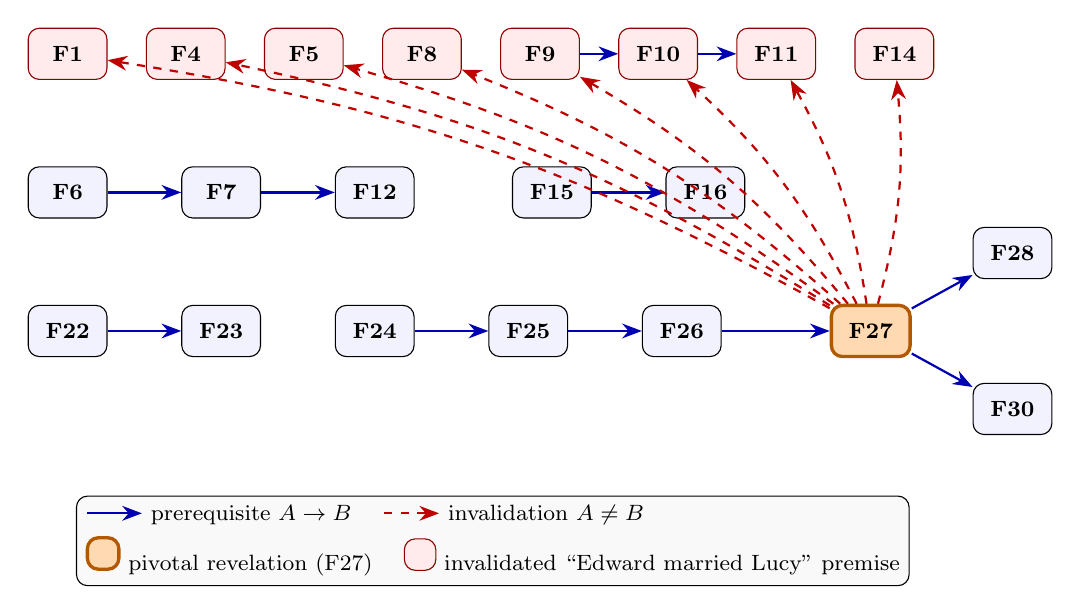
\begin{tikzpicture}[
    >={Stealth[length=2.5mm]},
    x=15mm, y=11mm,
    nnode/.style={draw,rounded corners,minimum width=10mm,minimum height=6.5mm,
                  inner sep=1pt,font=\footnotesize\bfseries,fill=blue!5},
    pivot/.style={nnode,fill=orange!30,draw=orange!70!black,very thick},
    falsey/.style={nnode,fill=red!8,draw=red!55!black},
    prereq/.style={->,blue!70!black,thick},
    invalid/.style={->,red!75!black,dashed,thick},
  ]

  % Layout: invalidated premises along the TOP row (the false "Edward married
  % Lucy" thread), the live event chain along the MIDDLE/BOTTOM, F27 at the
  % pivot on the right. Generous, uniform spacing prevents any overlap.

  % --- top row: the invalidated premises (tinted red) ---
  \node[falsey] (f1)  at (0,4)  {F1};
  \node[falsey] (f4)  at (1,4)  {F4};
  \node[falsey] (f5)  at (2,4)  {F5};
  \node[falsey] (f8)  at (3,4)  {F8};
  \node[falsey] (f9)  at (4,4)  {F9};
  \node[falsey] (f10) at (5,4)  {F10};
  \node[falsey] (f11) at (6,4)  {F11};
  \node[falsey] (f14) at (7,4)  {F14};

  % --- supposition chain (just below the top row, left) ---
  \draw[prereq] (f9)  -- (f10);
  \draw[prereq] (f10) -- (f11);

  % --- arrival sub-chain (upper-middle, left) ---
  \node[nnode] (f6)  at (0,2.4) {F6};
  \node[nnode] (f7)  at (1.3,2.4) {F7};
  \node[nnode] (f12) at (2.6,2.4) {F12};
  \draw[prereq] (f6) -- (f7);
  \draw[prereq] (f7) -- (f12);

  % --- retreat ---
  \node[nnode] (f15) at (4.1,2.4) {F15};
  \node[nnode] (f16) at (5.4,2.4) {F16};
  \draw[prereq] (f15) -- (f16);

  % --- dialogue / discovery chain (middle row) ---
  \node[nnode] (f22) at (0,0.8)   {F22};
  \node[nnode] (f23) at (1.3,0.8) {F23};
  \node[nnode] (f24) at (2.6,0.8) {F24};
  \node[nnode] (f25) at (3.9,0.8) {F25};
  \node[nnode] (f26) at (5.2,0.8) {F26};
  \draw[prereq] (f22) -- (f23);
  \draw[prereq] (f24) -- (f25);
  \draw[prereq] (f25) -- (f26);

  % --- the pivot and its consequences (bottom-right) ---
  \node[pivot] (f27) at (6.8,0.8)  {F27};
  \node[nnode] (f28) at (8.0,1.7)  {F28};
  \node[nnode] (f30) at (8.0,-0.1) {F30};
  \draw[prereq] (f26) -- (f27);
  \draw[prereq] (f27) -- (f28);
  \draw[prereq] (f27) -- (f30);

  % --- invalidation edges: F27 fans up to each false premise on the top row.
  %     A gentle uniform rightward bend keeps the eight dashed edges parallel
  %     and clear of the node labels. ---
  \foreach \t in {f1,f4,f5,f8,f9,f10,f11,f14} {
    \draw[invalid] (f27) to[bend right=10] (\t);
  }

  % --- legend ---
  \node[draw,fill=gray!5,rounded corners,anchor=north,align=left,
        font=\footnotesize] at (3.6,-1.1) {
    \tikz\draw[prereq](0,0)--(7mm,0);~prerequisite $A\rightarrow B$
    \quad
    \tikz\draw[invalid](0,0)--(7mm,0);~invalidation $A\neq B$\\[3pt]
    \tikz\node[pivot,minimum width=4mm,minimum height=4mm]{};~pivotal revelation (F27)
    \quad
    \tikz\node[falsey,minimum width=4mm,minimum height=4mm]{};~invalidated ``Edward married Lucy'' premise
  };

\end{tikzpicture}
\end{center}

\noindent\emph{(For legibility the graph shows the principal chains and the full
invalidation fan; purely sequential narration edges such as F1--F2 or F31--F32
are omitted. The mapping of these units onto the ground-truth scene below is
given in Table~\ref{tab:gt-align}, and the ground-truth dependency graph in
Figure~\ref{fig:gt-graph}.)}

\subsection*{Comparison against the ground-truth passage}

The paragraph analysed above is a paraphrase of the following \emph{ground-truth}
account of the same scene. We re-decompose the ground truth, align it to the
units F1--F33, and check that the relation structure (the pivot at the
``Robert married Lucy'' revelation, and the invalidation fan it triggers) is
preserved.

\noindent\textbf{Plain text.}
\begin{quote}
Elinor finds herself mulling over the event of Edward's marriage --- she realizes
that she'd hoped that something would come up to prevent it, but now that it's
happened, she feels incredibly hurt. She's surprised that he and Lucy were married
so soon, before he could possibly have been ordained. She wonders how he must have
felt, being so close to Barton. She supposes that the Ferrars must be settled at
Delaford already, and envisions their life there. Elinor had thought that someone
in London might have seen fit to tell her of Edward and Lucy's marriage, and she's
surprised when no letter arrives with details. She even asks her mother to write
to Colonel Brandon, eager for any news. However, no word has arrived. As soon as
she asks this, though, Colonel Brandon himself arrives --- but wait, it's not the
Colonel. In fact, it's Edward! Elinor tells herself to be calm. Marianne and
Mrs.~Dashwood both freak out as well, unsure of what they should do. They
silently await his arrival. Edward enters, looking ill with anxiety. Mrs.\
Dashwood breaks the ice by shaking his hand and wishing him happiness. Marianne
and Margaret both retreat, leaving Elinor and Mrs.~Dashwood to deal with the
visitor. Mrs.~Dashwood asks if Mrs.~Ferrars is well, and Elinor, following up,
asks if she's at Longstaple. Edward is shocked --- his mother isn't anywhere near
here! Elinor pointedly asks about Mrs.~Edward Ferrars. All eyes turn to Edward.
Edward stammers, confused --- does Elinor mean Mrs.~Robert Ferrars instead?
Everyone is shocked: what's the meaning of this? This is the deal --- it turns out
that Robert, Edward's younger brother, just married Lucy Steele. Whoa. Our minds
are blown. Elinor isn't sure how to react, so she flees the room and bursts into
tears of joy. Edward also doesn't know what to do, so he sits in silence for a
moment, then simply leaves. Everyone is totally perplexed.
\end{quote}

\noindent\textbf{Annotated.} Each highlighted clause is one ground-truth atomic
unit \textsuperscript{\textbf{\scriptsize G\textit{n}}}; the pivotal revelation
\textbf{G28} is orange. Casual interjections (``Whoa'', etc.) are not units.

\begin{quote}
\fu{cP1}{Elinor finds herself mulling over the event of Edward's marriage}{G1} --- she
\fu{cP2}{realizes that she'd hoped that something would come up to prevent it}{G2}, but now that it's
\fu{cP3}{happened, she feels incredibly hurt}{G3}.
\fu{cP4}{She's surprised that he and Lucy were married so soon}{G4},
\fu{cP5}{before he could possibly have been ordained}{G5}.
\fu{cP6}{She wonders how he must have felt, being so close to Barton}{G6}.
\fu{cP1}{She supposes that the Ferrars must be settled at Delaford already}{G7}, and
\fu{cP2}{envisions their life there}{G8}.
\fu{cP3}{Elinor had thought that someone in London might have seen fit to tell her of Edward and Lucy's marriage}{G9}, and she's
\fu{cP4}{surprised when no letter arrives with details}{G10}.
\fu{cP5}{She even asks her mother to write to Colonel Brandon, eager for any news}{G11}. However,
\fu{cP6}{no word has arrived}{G12}.
\fu{cP1}{As soon as she asks this, though, Colonel Brandon himself arrives}{G13} --- but wait, it's not the Colonel. In fact,
\fu{cP2}{it's Edward!}{G14} \fu{cP3}{Elinor tells herself to be calm}{G15}.
\fu{cP4}{Marianne and Mrs.~Dashwood both freak out as well, unsure of what they should do}{G16}.
\fu{cP5}{They silently await his arrival}{G17}.
\fu{cP6}{Edward enters, looking ill with anxiety}{G18}.
\fu{cP1}{Mrs.~Dashwood breaks the ice by shaking his hand and wishing him happiness}{G19}.
\fu{cP2}{Marianne and Margaret both retreat, leaving Elinor and Mrs.~Dashwood to deal with the visitor}{G20}.
\fu{cP3}{Mrs.~Dashwood asks if Mrs.~Ferrars is well}{G21}, and
\fu{cP4}{Elinor, following up, asks if she's at Longstaple}{G22}.
\fu{cP5}{Edward is shocked --- his mother isn't anywhere near here!}{G23}
\fu{cP6}{Elinor pointedly asks about Mrs.~Edward Ferrars}{G24}.
\fu{cP1}{All eyes turn to Edward}{G25}.
\fu{cP2}{Edward stammers, confused --- does Elinor mean Mrs.~Robert Ferrars instead?}{G26}
\fu{cP3}{Everyone is shocked: what's the meaning of this?}{G27} This is the deal --- it turns out that
\fu{cPivot}{Robert, Edward's younger brother, just married Lucy Steele}{G28}. Whoa. Our minds are blown.
\fu{cP5}{Elinor isn't sure how to react, so she flees the room and bursts into tears of joy}{G29}.
\fu{cP6}{Edward also doesn't know what to do, so he sits in silence for a moment, then simply leaves}{G30}.
\fu{cP1}{Everyone is totally perplexed}{G31}.
\end{quote}

\paragraph{Ground-truth atomic units (self-contained, in order of appearance).}
\begin{enumerate}[label=\textbf{G\arabic*.},leftmargin=*]
  \item Elinor mulls over the event of Edward's marriage.
  \item Elinor realizes she had hoped something would come up to prevent Edward's marriage.
  \item Elinor feels incredibly hurt now that Edward's marriage has happened.
  \item Elinor is surprised that Edward and Lucy were married so soon.
  \item Edward and Lucy were married before Edward could possibly have been ordained.
  \item Elinor wonders how Edward must have felt being so close to Barton.
  \item Elinor supposes that the Ferrars must be settled at Delaford already.
  \item Elinor envisions the Ferrars' life at Delaford.
  \item Elinor had thought someone in London might tell her of Edward and Lucy's marriage.
  \item Elinor is surprised when no letter arrives with details of the marriage.
  \item Elinor asks her mother to write to Colonel Brandon for news.
  \item No word has arrived from Colonel Brandon.
  \item As soon as Elinor asks, a visitor arrives and is taken to be Colonel Brandon.
  \item The visitor is in fact Edward, not Colonel Brandon.
  \item Elinor tells herself to be calm.
  \item Marianne and Mrs.~Dashwood are alarmed and unsure what to do.
  \item Marianne and Mrs.~Dashwood silently await Edward's arrival.
  \item Edward enters the room looking ill with anxiety.
  \item Mrs.~Dashwood breaks the ice by shaking Edward's hand and wishing him happiness.
  \item Marianne and Margaret retreat, leaving Elinor and Mrs.~Dashwood with the visitor.
  \item Mrs.~Dashwood asks whether Mrs.~Ferrars is well.
  \item Elinor asks whether Mrs.~Ferrars is at Longstaple.
  \item Edward is shocked because Edward's mother is not anywhere near Barton.
  \item Elinor pointedly asks about Mrs.~Edward Ferrars.
  \item All eyes turn to Edward.
  \item Edward, confused, asks whether Elinor means Mrs.~Robert Ferrars instead.
  \item Everyone is shocked and asks the meaning of this.
  \item Robert, Edward's younger brother, just married Lucy Steele.
  \item Elinor, unsure how to react, flees the room and bursts into tears of joy.
  \item Edward, unsure what to do, sits in silence and then leaves.
  \item Everyone is totally perplexed.
\end{enumerate}

\paragraph{Alignment to F1--F33.}
Table~\ref{tab:gt-align} maps each predicted unit to its ground-truth
counterpart. The two decompositions agree on the scene's content; the ground
truth additionally makes explicit two facts the paraphrase dropped --- that the
marriage preceded Edward's ordination (\textbf{G5}) and that Robert is
\emph{Edward's younger brother} (sharpening \textbf{G28} vs.\ predicted F27).

\begin{table}[h]
\centering\small
\begin{tabular}{lll}
\hline
\textbf{Predicted} & \textbf{Ground truth} & \textbf{Note}\\
\hline
F1, F14            & G10, G9        & awaited / missing news of the marriage\\
F4                 & G2             & hoped to prevent it\\
F5                 & G3             & feels hurt\\
F8                 & G4             & surprised married so soon\\
F9                 & G1             & mulls over the marriage\\
F10, F11           & G7, G8         & Delaford supposition / envisioned life\\
F2                 & G6             & wonders about Barton\\
F3                 & G11            & asks mother to write to Brandon\\
F20                & G12            & no word from Brandon\\
F6, F7             & G13, G14       & ``Brandon'' arrives $\to$ is Edward\\
F12               & G18            & Edward enters, ill with anxiety\\
F13                & G15            & Elinor tells herself to be calm\\
F17                & G16, G17       & others alarmed; silently await\\
F18, F19           & G19            & Mrs.~Dashwood greets / wishes happiness\\
F15, F16           & G20            & Marianne \& Margaret retreat\\
F21                & G21            & asks if Mrs.~Ferrars is well\\
F22                & G22            & asks if at Longstaple\\
F23                & G23            & Edward shocked: mother not near\\
F24                & G24            & pointed ``Mrs.~Edward Ferrars''\\
F25, F26           & G26 (+G25)     & confused; ``Mrs.~Robert Ferrars?''\\
\textbf{F27}       & \textbf{G28}   & \emph{pivot}: Robert (Edward's brother) married Lucy\\
F28                & G27            & everyone shocked\\
F29, F30           & G29            & Elinor flees; tears of joy\\
F31, F32           & G30            & Edward silent, then leaves\\
F33                & G31            & everyone perplexed\\
--                 & \textbf{G5}    & \emph{ground-truth only}: married before ordination\\
\hline
\end{tabular}
\caption{Alignment of the predicted units F1--F33 to the ground-truth units
G1--G31. Bold marks the shared pivot.}
\label{tab:gt-align}
\end{table}

\paragraph{Ground-truth dependency graph.}
Figure~\ref{fig:gt-graph} draws the relations on the ground-truth units, using
the same conventions as the predicted graph above. The structure is preserved:
\textbf{G28} (Robert married Lucy) is the pivot, and it invalidates exactly the
units that presuppose ``Edward married Lucy'' (G1--G4, G7--G10) --- the same
premise set as the predicted F27 fan. The extra ground-truth fact \textbf{G5}
(``married before ordination'') is likewise invalidated, since the marriage it
describes is Edward's.

\begin{figure}[h]
\centering
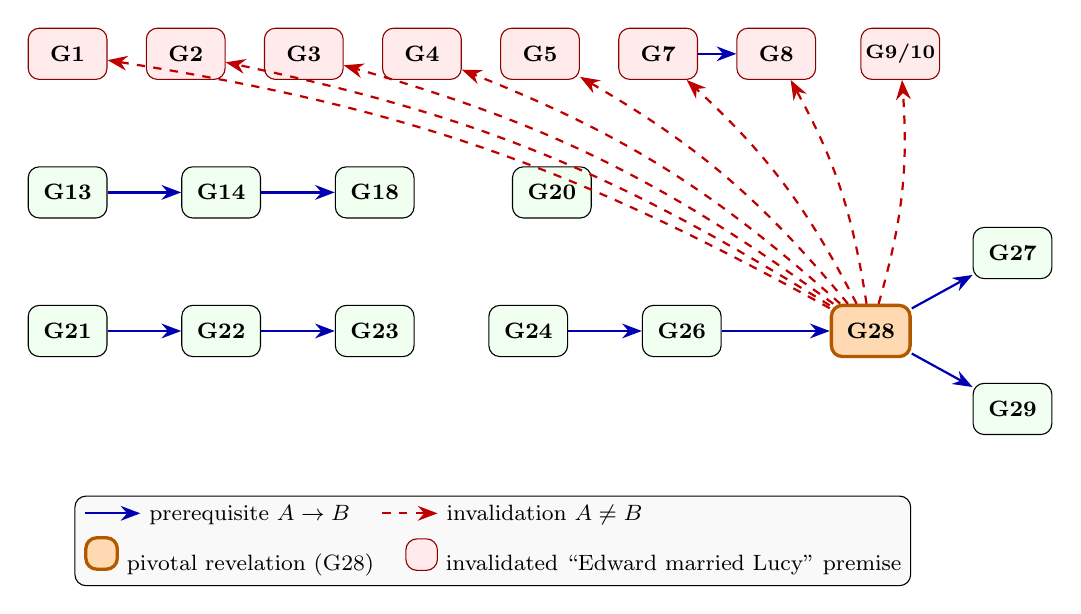
\begin{tikzpicture}[
    >={Stealth[length=2.5mm]},
    x=15mm, y=11mm,
    nnode/.style={draw,rounded corners,minimum width=10mm,minimum height=6.5mm,
                  inner sep=1pt,font=\footnotesize\bfseries,fill=green!6},
    pivot/.style={nnode,fill=orange!30,draw=orange!70!black,very thick},
    falsey/.style={nnode,fill=red!8,draw=red!55!black},
    prereq/.style={->,blue!70!black,thick},
    invalid/.style={->,red!75!black,dashed,thick},
  ]

  % --- top row: invalidated "Edward married Lucy" premises (incl. G5) ---
  \node[falsey] (g1)  at (0,4)  {G1};
  \node[falsey] (g2)  at (1,4)  {G2};
  \node[falsey] (g3)  at (2,4)  {G3};
  \node[falsey] (g4)  at (3,4)  {G4};
  \node[falsey] (g5)  at (4,4)  {G5};
  \node[falsey] (g7)  at (5,4)  {G7};
  \node[falsey] (g8)  at (6,4)  {G8};
  \node[falsey] (g910) at (7.05,4) {\scriptsize G9/10};

  % --- supposition chain ---
  \draw[prereq] (g7) -- (g8);

  % --- arrival sub-chain ---
  \node[nnode] (g13) at (0,2.4)   {G13};
  \node[nnode] (g14) at (1.3,2.4) {G14};
  \node[nnode] (g18) at (2.6,2.4) {G18};
  \draw[prereq] (g13) -- (g14);
  \draw[prereq] (g14) -- (g18);

  % --- retreat ---
  \node[nnode] (g20) at (4.1,2.4) {G20};

  % --- dialogue / discovery chain ---
  \node[nnode] (g21) at (0,0.8)   {G21};
  \node[nnode] (g22) at (1.3,0.8) {G22};
  \node[nnode] (g23) at (2.6,0.8) {G23};
  \node[nnode] (g24) at (3.9,0.8) {G24};
  \node[nnode] (g26) at (5.2,0.8) {G26};
  \draw[prereq] (g21) -- (g22);
  \draw[prereq] (g22) -- (g23);
  \draw[prereq] (g24) -- (g26);

  % --- pivot + consequences ---
  \node[pivot] (g28) at (6.8,0.8)  {G28};
  \node[nnode] (g27) at (8.0,1.7)  {G27};
  \node[nnode] (g29) at (8.0,-0.1) {G29};
  \draw[prereq] (g26) -- (g28);
  \draw[prereq] (g28) -- (g27);
  \draw[prereq] (g28) -- (g29);

  % --- invalidation fan from the pivot ---
  \foreach \t in {g1,g2,g3,g4,g5,g7,g8,g910} {
    \draw[invalid] (g28) to[bend right=10] (\t);
  }

  % --- legend ---
  \node[draw,fill=gray!5,rounded corners,anchor=north,align=left,
        font=\footnotesize] at (3.6,-1.1) {
    \tikz\draw[prereq](0,0)--(7mm,0);~prerequisite $A\rightarrow B$
    \quad
    \tikz\draw[invalid](0,0)--(7mm,0);~invalidation $A\neq B$\\[3pt]
    \tikz\node[pivot,minimum width=4mm,minimum height=4mm]{};~pivotal revelation (G28)
    \quad
    \tikz\node[falsey,minimum width=4mm,minimum height=4mm]{};~invalidated ``Edward married Lucy'' premise
  };

\end{tikzpicture}
\caption{Ground-truth dependency graph (units G1--G31). The pivot \textbf{G28}
mirrors the predicted pivot F27 (Table~\ref{tab:gt-align}); its invalidation fan
covers the same premise set, plus the ground-truth-only unit G5 (married before
ordination).}
\label{fig:gt-graph}
\end{figure}

\subsection*{Temporal-order discrepancies}

The ground-truth units \textbf{G1--G31 are listed in chronological order}: G$i$
happens before G$j$ whenever $i<j$. The altered passage, however, narrates the
\emph{same} events in a different order. Using the alignment of
Table~\ref{tab:gt-align}, we assign each predicted unit its
\emph{chronological rank} (the index of the ground-truth event it reports) and
ask whether reading F1, F2, \dots, F33 in order visits those ranks in increasing
order. Wherever a later predicted unit reports an \emph{earlier} event than one
before it, the narration has jumped backwards in time --- a temporal
discrepancy.

\paragraph{Chronological rank of each predicted unit.}
\begin{center}\small
\begin{tabular}{l*{17}{c}}
\hline
F  & 1&2&3&4&5&6&7&8&9&10&11&12&13&14&15&16&17\\
rank (G) & 10&6&11&2&3&13&14&4&\textbf{1}&7&8&18&15&9&20&20&16\\
\hline
F  & 18&19&20&21&22&23&24&25&26&27&28&29&30&31&32&33&\\
rank (G) & 19&19&\textbf{12}&21&22&23&24&25&26&\textbf{28}&\textbf{27}&29&29&30&30&31&\\
\hline
\end{tabular}
\end{center}

In a perfectly ordered paraphrase this rank sequence would be non-decreasing.
Instead it lurches: it opens at rank~10, drops to rank~2 (F4), reaches back to
rank~\textbf{1} at F9 (the chronological \emph{start} of the scene, narrated
ninth), and only settles into order from F21 onward. Two discrepancies survive
into the otherwise-ordered tail: F20 (rank~12, the missing word from Brandon,
displaced very late) and the climactic local swap F27/F28
(rank~28 before rank~27).

\paragraph{What is out of place.}
\begin{itemize}[leftmargin=*]
  \item \textbf{Scrambled opening cluster (F1--F14).} Chronologically the scene
        runs G1\,(mulls)$\to$G2\,(hoped to prevent)$\to$G3\,(hurt)$\to$
        G4\,(so soon)$\to$G6\,(Barton)$\to$G7/8\,(Delaford)$\to$
        G9/10\,(London / no letter)$\to$G11\,(asks mother)$\to$G12\,(no word).
        The paraphrase instead \emph{opens} with the missing-letter surprise
        (F1$=$G10) and the Barton musing (F2$=$G6), asks the mother (F3$=$G11)
        \emph{before} establishing the hurt (F4/F5$=$G2/G3), and reaches the true
        starting beat ``Elinor mulls over the marriage'' (F9$=$G1) only ninth.
  \item \textbf{Displaced ``no word from Brandon'' (F20$=$G12).} In the ground
        truth this immediately follows the request to write (G11); the paraphrase
        moves it past the arrival and greeting, to just before Mrs.~Dashwood's
        question about Mrs.~Ferrars.
  \item \textbf{Climactic swap (F27$\leftrightarrow$F28, i.e.\ G28 before G27).}
        The paraphrase states the revelation (Robert married Lucy) and then
        reports the general shock; the ground truth has the shocked
        ``what's the meaning of this?'' (G27) precede the explanatory reveal
        (G28).
\end{itemize}

\paragraph{Discrepancy plot.}
Figure~\ref{fig:order} plots each predicted unit at $(\text{appearance order},
\text{chronological rank})$. A faithful retelling would lie on the rising dotted
diagonal; every point \emph{below} that diagonal is an event told later than its
true time, and every \textbf{red back-arc} connects consecutive units where the
story jumps backwards in time. The dense tangle of back-arcs over F1--F14 is the
scrambled opening; the lone late arcs are F20 and the F27/F28 swap.

\begin{figure}[h]
\centering
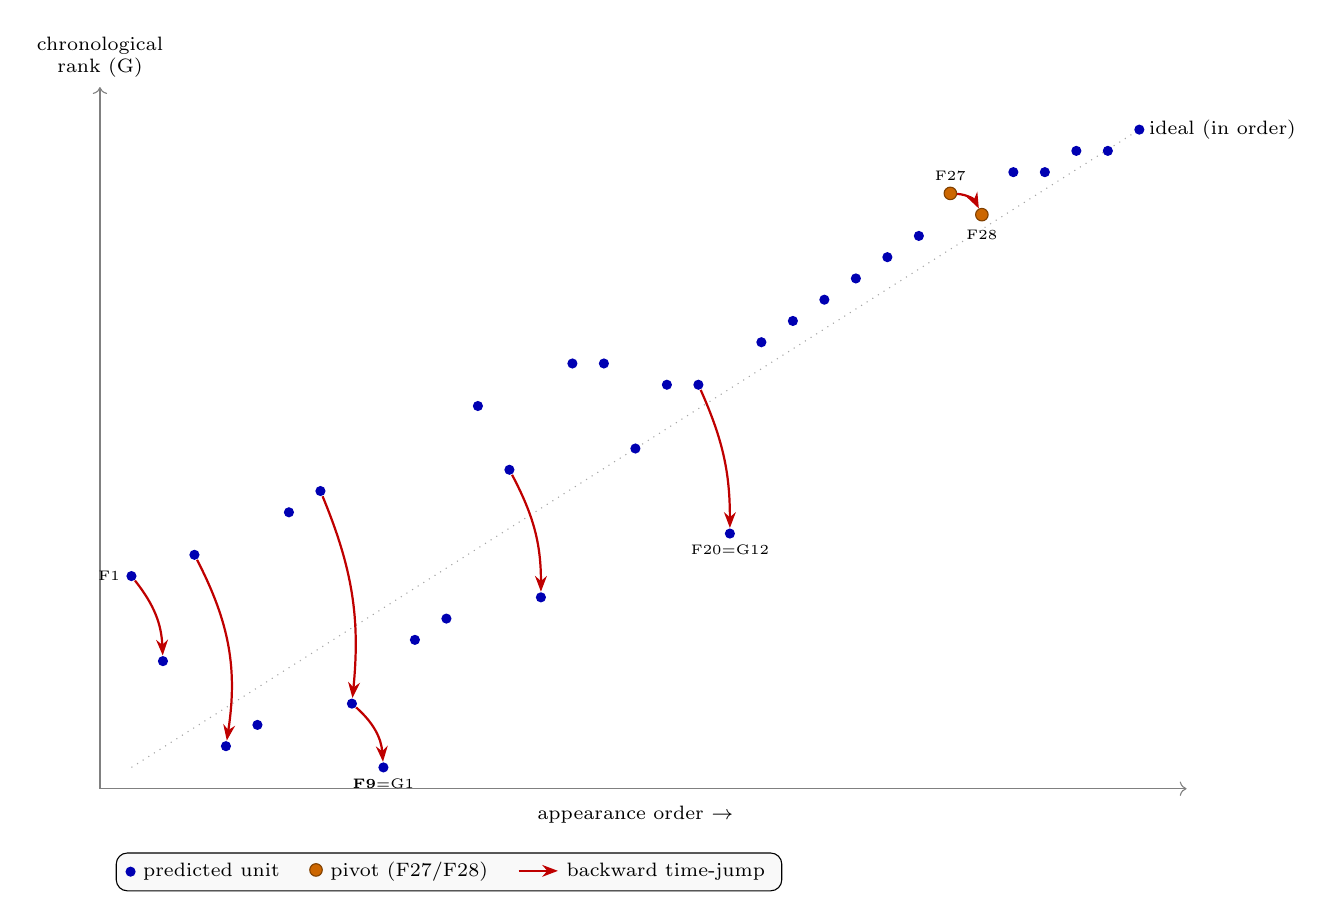
\begin{tikzpicture}[
    x=4.0mm, y=2.7mm,
    dot/.style={circle,fill=blue!70!black,inner sep=1.3pt},
    pdot/.style={circle,fill=orange!80!black,draw=orange!50!black,inner sep=1.6pt},
    back/.style={->,red!75!black,thick,>={Stealth[length=2mm]}},
    lbl/.style={font=\tiny,inner sep=1pt},
  ]

  % axes
  \draw[->,gray] (0,0) -- (34.5,0);
  \node[font=\scriptsize,below=1mm] at (17,0) {appearance order $\rightarrow$};
  \draw[->,gray] (0,0) -- (0,33) node[above,font=\scriptsize,black,align=center] {chronological\\rank (G)};
  % ideal diagonal: rank == position would be perfect; scale 31 ranks over 33 slots
  \draw[dotted,gray!70] (1,1) -- (33,31) node[right,font=\scriptsize,black] {ideal (in order)};

  % data: (Findex, chronoRank); pivot F27/F28 in orange
  \foreach \i/\r in {1/10,2/6,3/11,4/2,5/3,6/13,7/14,8/4,9/1,10/7,11/8,
                     12/18,13/15,14/9,15/20,16/20,17/16,18/19,19/19,20/12,
                     21/21,22/22,23/23,24/24,25/25,26/26,29/29,30/29,
                     31/30,32/30,33/31}
    \node[dot] (p\i) at (\i,\r) {};
  \node[pdot] (p27) at (27,28) {};
  \node[pdot] (p28) at (28,27) {};

  % label a few salient points
  \node[lbl,below=1pt of p9]  {\textbf{F9}=G1};
  \node[lbl,left=1pt of p1]   {F1};
  \node[lbl,below=1pt of p20] {F20=G12};
  \node[lbl,above=1pt of p27] {F27};
  \node[lbl,below=2pt of p28] {F28};

  % red back-arcs: consecutive F where chronological rank decreases
  % opening scramble
  \draw[back] (p1) to[bend left=18] (p2);    % 10 -> 6
  \draw[back] (p3) to[bend left=18] (p4);    % 11 -> 2
  \draw[back] (p7) to[bend left=14] (p8);    % 14 -> 4
  \draw[back] (p8) to[bend left=22] (p9);    % 4  -> 1
  \draw[back] (p13) to[bend left=14] (p14);  % 15 -> 9
  % late displacements
  \draw[back] (p19) to[bend left=12] (p20);  % 19 -> 12
  \draw[back] (p27) to[bend left=30] (p28);  % 28 -> 27 (climactic swap)

  % legend
  \node[draw,fill=gray!5,rounded corners,anchor=north west,align=left,
        font=\scriptsize] at (0.5,-3) {
    \tikz\node[dot]{}; predicted unit \quad
    \tikz\node[pdot]{}; pivot (F27/F28) \quad
    \tikz\draw[back](0,0)--(5mm,0); backward time-jump
  };

\end{tikzpicture}
\caption{Temporal-order discrepancy plot. Each predicted unit F$i$ is placed at
its appearance order ($x$) and the chronological rank of the ground-truth event
it reports ($y$). A faithful retelling tracks the dotted diagonal; points below
it are told late, and red arcs mark consecutive backward jumps in time. The
opening cluster F1--F14 is badly scrambled (it reaches the true first event,
F9$=$G1, only ninth), while F21--F33 is ordered apart from the displaced F20 and
the climactic F27/F28 swap.}
\label{fig:order}
\end{figure}

% =============================================================================
\section{Fourth example: synthesizing a summary from a reliable and an
unreliable source}

This example starts from two source paragraphs about the same subject. Source
\textbf{A} is largely accurate; source \textbf{B} is a sensational news piece
containing several factual errors that \emph{contradict} A. We then synthesize a
summary \textbf{S} that deliberately interleaves claims from both, so that S
contains both logical-implication chains and positional invalidations, and we
analyse S with the usual decomposition.

\subsection*{Source A (reliable)}
\begin{quote}\small
Keyara Jones is an American college basketball player who played in the NCAA
Division I women's basketball league. Jones played college basketball for the
University of Alabama during the 2020--2021 season, as a member of the Crimson
Tide women's basketball team, which competes in the Southeastern Conference (SEC)
of NCAA Division I. The NCAA Division I women's basketball league consists of 356
teams and is considered the highest level of women's college basketball in the
United States. According to the University of Alabama's athletic website, Jones
is listed as a \emph{guard from Birmingham, Alabama}, and was a member of the
women's basketball team during the 2020--2021 season; ESPN and CBS Sports also
reported on her performances that season.
\end{quote}

\subsection*{Source B (unreliable --- contains factual errors)}
\begin{quote}\small
``Breaking News: Alabama's Keyara Jones Makes History as First Female Player in
NCAA Division~I \emph{Men's} Basketball.'' The 20-year-old junior, a 5$'$10$''$
\emph{guard from Montgomery, Alabama}, made her debut last night. Averaging 18
points and 7 rebounds per game, she led the Alabama women's team to a Sweet~16
appearance last season. Coach Nate Oats praised her, and a sports sociologist
called it a milestone for gender equality. ``According to NCAA data, only 12\% of
Division~I men's basketball players are women,'' the piece reports, framing
Jones' entry as a step toward greater gender representation; several NBA teams
are said to be scouting her.
\end{quote}

\noindent
\textbf{Errors in B (each contradicts A).} (i)~Jones joined an NCAA Division~I
\emph{men's} team --- A has her on the \emph{women's} team. (ii)~She is a guard
from \emph{Montgomery} --- A's cited source says \emph{Birmingham}.
(iii)~The ``12\% of men's players are women'' statistic is internally absurd.
The fabricated junior/height/Sweet~16/NBA-scouting details have no support in A.

\subsection*{Synthesized summary S}

S is written to interleave B's sensational (false) framing \emph{first} with A's
reliable record \emph{afterward}, so that the later (true) atoms positionally
invalidate the earlier (false) ones, while several implication chains run within
each block.

\noindent\textbf{Plain text.}
\begin{quote}
Keyara Jones is an American college basketball player from Montgomery, Alabama,
who plays guard for the University of Alabama. During the 2020--2021 season she
made history as the first woman to join an NCAA Division~I men's basketball team,
averaging 18 points per game and leading Alabama to a Sweet~16 appearance.
Because she competed in the men's league, her achievement was hailed as a
milestone for gender equality, and NCAA data showing that 12\% of Division~I
men's players are women was cited to underscore the trend. In fact, the
University of Alabama's athletic website lists Jones as a guard from Birmingham,
Alabama, who was a member of the women's basketball team during the 2020--2021
season. The Crimson Tide women's team competes in the Southeastern Conference of
NCAA Division~I women's basketball, which is the highest level of women's college
basketball in the United States and consists of 356 teams.
\end{quote}

\noindent\textbf{Annotated.} Each clause is one atomic unit
\textsuperscript{\textbf{\scriptsize S\textit{n}}}. Red marks a false atom
imported from source~B, green a reliable atom from source~A; neutral (blue) atoms
are uncontested.

\begin{quote}
\fu{cId}{Keyara Jones is an American college basketball player}{S1}
\fu{cLate}{from Montgomery, Alabama}{S2},
\fu{cId}{who plays guard for the University of Alabama}{S3}. During the
2020--2021 season she
\fu{cLate}{made history as the first woman to join an NCAA Division~I men's basketball team}{S4},
\fu{cId}{averaging 18 points per game}{S5} and
\fu{cId}{leading Alabama to a Sweet~16 appearance}{S6}. Because she
\fu{cLate}{competed in the men's league}{S7},
\fu{cLate}{her achievement was hailed as a milestone for gender equality}{S8}, and
\fu{cLate}{NCAA data showing that 12\% of Division~I men's players are women}{S9}
\fu{cLate}{was cited to underscore the trend}{S10}. In fact, the
\fu{cEarly}{University of Alabama's athletic website lists Jones as a guard from Birmingham, Alabama}{S11},
\fu{cEarly}{who was a member of the women's basketball team during the 2020--2021 season}{S12}.
\fu{cEarly}{The Crimson Tide women's team competes in the Southeastern Conference of NCAA Division~I women's basketball}{S13},
\fu{cEarly}{which is the highest level of women's college basketball in the United States}{S14} and
\fu{cEarly}{consists of 356 teams}{S15}.
\end{quote}

\subsection*{Atomic units of S (self-contained, in order of appearance)}
\begin{enumerate}[label=\textbf{S\arabic*.},leftmargin=*]
  \item Keyara Jones is an American college basketball player.
  \item Keyara Jones is from Montgomery, Alabama.
  \item Keyara Jones plays guard for the University of Alabama.
  \item During the 2020--2021 season Keyara Jones made history as the first woman to join an NCAA Division~I men's basketball team.
  \item Keyara Jones averaged 18 points per game.
  \item Keyara Jones led Alabama to a Sweet~16 appearance.
  \item Keyara Jones competed in the men's basketball league.
  \item Keyara Jones' achievement was hailed as a milestone for gender equality.
  \item NCAA data show that 12\% of Division~I men's basketball players are women.
  \item The 12\% statistic was cited to underscore the gender-equality trend.
  \item The University of Alabama's athletic website lists Keyara Jones as a guard from Birmingham, Alabama.
  \item Keyara Jones was a member of the University of Alabama women's basketball team during the 2020--2021 season.
  \item The Crimson Tide women's team competes in the Southeastern Conference of NCAA Division~I women's basketball.
  \item NCAA Division~I women's basketball is the highest level of women's college basketball in the United States.
  \item NCAA Division~I women's basketball consists of 356 teams.
\end{enumerate}

\subsection*{Relations}

\textbf{Logical prerequisites ($A \rightarrow B$).}
\begin{itemize}[leftmargin=*]
  \item S3 $\rightarrow$ S4 --- playing for Alabama is presupposed by joining an Alabama (men's) team.
  \item S4 $\rightarrow$ S7 --- joining a men's team is what it means to compete in the men's league.
  \item S7 $\rightarrow$ S8 --- competing in the men's league is the stated ground for the gender-equality acclaim.
  \item S9 $\rightarrow$ S10 --- the 12\% statistic is what is cited to underscore the trend.
  \item S8,\,S10 share the gender-equality framing (S10 reinforces S8).
  \item S12 $\rightarrow$ S13 --- membership of the women's team is presupposed by that team competing in the SEC.
  \item S13 $\rightarrow$ S14 --- the women's league existing/being top-level is presupposed by S13 placing the team in it.
  \item S14 $\rightarrow$ S15 --- the league being characterised (top level) is presupposed by counting its 356 teams.
  \item S1 $\rightarrow$ S3 --- being a college basketball player is presupposed by playing guard for a specific program.
\end{itemize}

\noindent
\textbf{Position invalidations ($A \neq B$).} The reliable atoms S11 and S12
(from source A), appearing \emph{after} B's framing, positionally invalidate the
earlier false atoms.

\begin{itemize}[leftmargin=*]
  \item S11 $\neq$ S2 --- the cited website says \emph{Birmingham}, contradicting ``from Montgomery.''
  \item S12 $\neq$ S4 --- being on the \emph{women's} team contradicts ``first woman on a men's team.''
  \item S12 $\neq$ S7 --- women's-team membership contradicts ``competed in the men's league.''
  \item S12 $\neq$ S8 --- with no men's-league entry, the gender-equality milestone collapses.
  \item S12 $\neq$ S10 --- the men's-representation framing is voided once the men's-league premise fails.
  \item S9 $\neq$ S9 (self-inconsistent) --- ``12\% of \emph{men's} players are women'' is internally contradictory regardless of position.
\end{itemize}

\noindent
\textbf{Note.} The Sweet~16 and 18-ppg atoms (S5, S6) are unsupported by A but
not directly contradicted by it; they are left as neither implied nor
invalidated. The contradiction structure is concentrated on S12 (true
women's-team membership) overturning the men's-league thread S4--S10.

\subsection*{Relation graph}

Solid blue arrows are logical prerequisites ($A \rightarrow B$); dashed red
arrows are position invalidations ($A \neq B$). False atoms imported from B are
tinted red; the two reliable invalidating atoms from A (S11, S12) are green and
highlighted. The self-contradictory statistic S9 carries a red self-loop.

\begin{center}
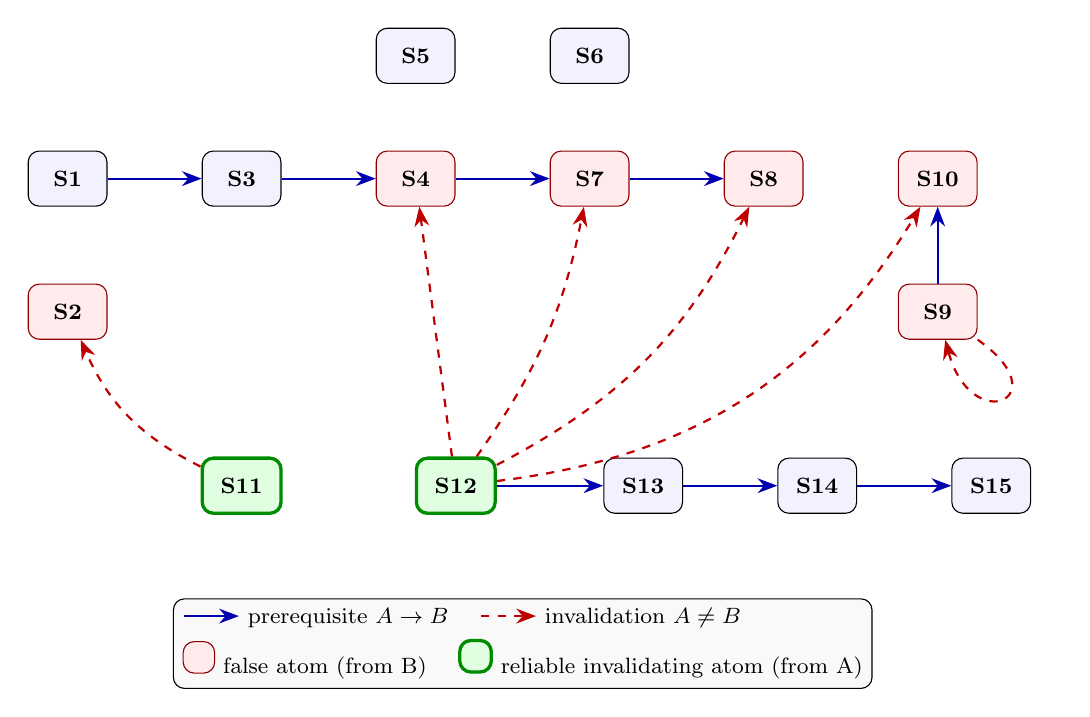
\begin{tikzpicture}[
    >={Stealth[length=2.5mm]},
    x=17mm, y=13mm,
    snode/.style={draw,rounded corners,minimum width=10mm,minimum height=7mm,
                  inner sep=1pt,font=\footnotesize\bfseries,fill=blue!5},
    falsey/.style={snode,fill=red!8,draw=red!55!black},
    truthy/.style={snode,fill=green!12,draw=green!55!black,very thick},
    prereq/.style={->,blue!70!black,thick},
    invalid/.style={->,red!75!black,dashed,thick},
  ]

  % --- top: B's false "men's league" thread (left to right) ---
  \node[snode]  (s1) at (0,3)   {S1};
  \node[falsey] (s2) at (0,1.7) {S2};
  \node[snode]  (s3) at (1.3,3) {S3};
  \node[falsey] (s4) at (2.6,3) {S4};
  \node[falsey] (s7) at (3.9,3) {S7};
  \node[falsey] (s8) at (5.2,3) {S8};
  \node[falsey] (s10) at (6.5,3) {S10};
  \node[falsey] (s9)  at (6.5,1.7) {S9};

  % --- unsupported (neither) ---
  \node[snode]  (s5) at (2.6,4.2) {S5};
  \node[snode]  (s6) at (3.9,4.2) {S6};

  % --- bottom: A's reliable thread ---
  \node[truthy] (s11) at (1.3,0)  {S11};
  \node[truthy] (s12) at (2.9,0)  {S12};
  \node[snode]  (s13) at (4.3,0)  {S13};
  \node[snode]  (s14) at (5.6,0)  {S14};
  \node[snode]  (s15) at (6.9,0)  {S15};

  % --- prerequisite edges ---
  \draw[prereq] (s1) -- (s3);
  \draw[prereq] (s3) -- (s4);
  \draw[prereq] (s4) -- (s7);
  \draw[prereq] (s7) -- (s8);
  \draw[prereq] (s9) -- (s10);
  \draw[prereq] (s12) -- (s13);
  \draw[prereq] (s13) -- (s14);
  \draw[prereq] (s14) -- (s15);

  % --- invalidation edges from the reliable atoms ---
  \draw[invalid] (s11) to[bend left=20] (s2);
  \draw[invalid] (s12) -- (s4);
  \draw[invalid] (s12) to[bend right=12] (s7);
  \draw[invalid] (s12) to[bend right=18] (s8);
  \draw[invalid] (s12) to[bend right=26] (s10);

  % --- self-contradiction loop on S9 ---
  \draw[invalid] (s9) to[out=-35,in=-75,looseness=8] (s9);

  % --- legend ---
  \node[draw,fill=gray!5,rounded corners,anchor=north,align=left,
        font=\footnotesize] at (3.4,-1.1) {
    \tikz\draw[prereq](0,0)--(7mm,0);~prerequisite $A\rightarrow B$
    \quad
    \tikz\draw[invalid](0,0)--(7mm,0);~invalidation $A\neq B$\\[3pt]
    \tikz\node[falsey,minimum width=4mm,minimum height=4mm]{};~false atom (from B)
    \quad
    \tikz\node[truthy,minimum width=4mm,minimum height=4mm]{};~reliable invalidating atom (from A)
  };

\end{tikzpicture}
\end{center}

\noindent\emph{(S5 and S6 --- the unsupported 18-ppg and Sweet~16 claims --- are
shown without relation edges: A neither implies nor contradicts them.)}

% =============================================================================
\section{Fifth example: a real legal case (\emph{R v Renda})}

This example applies the task to a genuine judgment: \emph{Renda, R v}
\mbox{[2005] EWCA Crim 2826} (England and Wales Court of Appeal, Criminal
Division, 10 November 2005; also reported at [2006] 1 WLR 2948), supplied as the
case file \texttt{clc/-ew-cases-EWCA-Crim-2005-2826.xml}. The judgment disposes
of six conjoined appeals on the ``bad character'' provisions of the Criminal
Justice Act 2003; we summarise the lead appeal, \textbf{Renda}, which contains
several factual tensions that the relation analysis brings out.

\subsection*{Source (provenance)}
\begin{quote}\small
Court of Appeal (Criminal Division), per the President of the Queen's Bench
Division (Sir Igor Judge). Appeal of Raymond Renda against conviction for
attempted robbery before HHJ Van Der Werff and a jury at the Inner London Crown
Court; the appeal turned on the Criminal Justice Act 2003 ``false impression''
(s\,101(1)(f), s\,105), ``reprehensible behaviour'' (s\,112) and
``contamination'' (s\,107) provisions.
\end{quote}

\subsection*{Synthesized summary S}

S states Renda's self-serving evidence \emph{first} and the conceded truths and
the court's holdings \emph{afterward}, so that the later atoms positionally
contradict the earlier ones, while prerequisite chains run from the charge
through to the dismissal.

\noindent\textbf{Plain text.}
\begin{quote}
Raymond Renda was convicted of attempted robbery and appealed against that
conviction. The charge arose when, at about 2~am on 10~November 2003, Renda
accosted Robert Flint on Mile End Road, followed him home, and seized him by the
neck demanding money; the trial turned on the relative credibility of Flint and
Renda. To enhance his credibility Renda testified to his good character: he
claimed that his serious head injury had been sustained while he was serving on
duty in the armed forces, and that he was currently in regular employment as a
security guard. In fact, as he conceded under cross-examination, the head injury
was sustained on holiday in a car accident, and his security work had been only
short-term pass-checking so that he was no longer employed; he had therefore
conveyed a false impression of positive good character. The defence argued that
this cross-examination concession withdrew the false impression under s\,105(3),
but the court held that a concession forced in cross-examination is not a
withdrawal. The court also recounted that in July~2001 Renda had been found unfit
to plead to assault and given an absolute discharge, so that he stood not
convicted, even though a jury had found as a fact that he struck a man from
behind with a wooden table leg, which the court held to be reprehensible
behaviour. Renda's counsel initially conceded that this table-leg finding
amounted to a conviction, then later concluded that it was not a conviction. The
court held that the evidence was not contaminated, and the appeal was dismissed.
\end{quote}

\noindent\textbf{Annotated.} Each clause is one atomic unit
\textsuperscript{\textbf{\scriptsize L\textit{n}}}. Colours match the relation
graph: blue~=~neutral fact, red~=~Renda's claim/position, green~=~conceded truth,
orange~=~court's holding.

\begin{quote}
\fu{cFact}{Raymond Renda was convicted of attempted robbery}{L1} and
\fu{cFact}{appealed against that conviction}{L2}. The charge arose when,
\fu{cFact}{at about 2~am on 10~November 2003, Renda accosted Robert Flint on Mile End Road, followed him home, and seized him by the neck demanding money}{L3};
\fu{cFact}{the trial turned on the relative credibility of Flint and Renda}{L4}.
\fu{cFact}{To enhance his credibility Renda testified to his good character}{L5}: he
\fu{cClaim}{claimed that his serious head injury had been sustained while he was serving on duty in the armed forces}{L6}, and that
\fu{cClaim}{he was currently in regular employment as a security guard}{L7}. In
fact, as he conceded under cross-examination,
\fu{cTruth}{the head injury was sustained on holiday in a car accident}{L8}, and
\fu{cTruth}{his security work had been only short-term pass-checking so that he was no longer employed}{L9};
\fu{cFact}{he had therefore conveyed a false impression of positive good character}{L10}.
\fu{cClaim}{The defence argued that this cross-examination concession withdrew the false impression under \mbox{s\,105(3)}}{L11}, but
\fu{cHold}{the court held that a concession forced in cross-examination is not a withdrawal}{L12}. The court also recounted that
\fu{cFact}{in July~2001 Renda had been found unfit to plead to assault and given an absolute discharge, so that he stood not convicted}{L13}, even though
\fu{cFact}{a jury had found as a fact that he struck a man from behind with a wooden table leg}{L14},
\fu{cHold}{which the court held to be reprehensible behaviour}{L15}.
\fu{cClaim}{Renda's counsel initially conceded that this table-leg finding amounted to a conviction}{L16},
\fu{cTruth}{then later concluded that it was not a conviction}{L17}.
\fu{cHold}{The court held that the evidence was not contaminated, and the appeal was dismissed}{L18}.
\end{quote}

\subsection*{Atomic units of S (self-contained, in order of appearance)}
\begin{enumerate}[label=\textbf{L\arabic*.},leftmargin=*]
  \item Raymond Renda was convicted of attempted robbery.
  \item Raymond Renda appealed against the attempted-robbery conviction.
  \item Renda accosted Robert Flint on Mile End Road at about 2~am on 10~November 2003 and seized him by the neck while demanding money.
  \item The trial turned on the relative credibility of Robert Flint and Raymond Renda.
  \item Renda testified to his good character in order to enhance his credibility.
  \item Renda claimed his serious head injury was sustained while he was serving on duty in the armed forces.
  \item Renda claimed he was currently in regular employment as a security guard.
  \item In fact Renda's serious head injury was sustained on holiday in a car accident.
  \item In fact Renda's security work had been only short-term pass-checking and he was no longer employed.
  \item Renda had conveyed a false impression of positive good character.
  \item The defence argued that Renda's cross-examination concession withdrew the false impression under s\,105(3).
  \item The court held that a concession forced in cross-examination is not a withdrawal of a false impression.
  \item In July~2001 Renda was found unfit to plead to assault and given an absolute discharge, so he stood not convicted.
  \item A jury found as a fact that Renda struck a man from behind with a wooden table leg.
  \item The court held that the table-leg incident was reprehensible behaviour.
  \item Renda's counsel initially conceded that the table-leg finding amounted to a conviction.
  \item Renda's counsel later concluded that the table-leg finding was not a conviction.
  \item The court held that the evidence was not contaminated and dismissed the appeal.
\end{enumerate}

\subsection*{Relations}

\textbf{Logical prerequisites ($A \rightarrow B$).}
\begin{itemize}[leftmargin=*]
  \item L1 $\rightarrow$ L2 --- a conviction is presupposed by an appeal against that conviction.
  \item L3 $\rightarrow$ L1 --- the attempted-robbery incident grounds the conviction for it.
  \item L4 $\rightarrow$ L5 --- the trial turning on credibility is why Renda testified to enhance his credibility.
  \item L5 $\rightarrow$ L6,\,L7 --- the good-character testimony comprises the two specific claims.
  \item L8,\,L9 $\rightarrow$ L10 --- the conceded truths are what establish that a false impression was conveyed.
  \item L10 $\rightarrow$ L11 --- the existence of a false impression is presupposed by arguing it was withdrawn.
  \item L13,\,L14 $\rightarrow$ L15 --- the unfit-to-plead finding plus the table-leg act ground the ``reprehensible behaviour'' holding.
  \item L12,\,L15 $\rightarrow$ L18 --- the holdings that defeated Renda's challenges ground the dismissal of the appeal.
\end{itemize}

\noindent
\textbf{Contradictions / position invalidations ($A \neq B$).} Each conceded
truth or holding, stated later, contradicts an earlier self-serving claim or
argument.
\begin{itemize}[leftmargin=*]
  \item L8 $\neq$ L6 --- injured on holiday in a car accident contradicts injured on duty in the armed forces.
  \item L9 $\neq$ L7 --- being no longer employed (short-term pass-checking) contradicts being currently in regular employment.
  \item L12 $\neq$ L11 --- the court's holding that a forced concession is not a withdrawal defeats the defence's s\,105(3) argument.
  \item L15 $\neq$ L13 --- ``reprehensible behaviour'' is held to stand despite there being no conviction, defeating the implied argument that no conviction means no reprehensible behaviour.
  \item L17 $\neq$ L16 --- counsel's later conclusion (not a conviction) contradicts her initial concession (a conviction).
\end{itemize}

\noindent
\textbf{Note.} The contradictions cluster on the credibility issue (Renda's
claims L6/L7 vs.\ the conceded truths L8/L9) and on two reversed legal positions
(L11/L12 and L16/L17), plus the not-convicted-vs.-reprehensible tension
(L13/L15). The prerequisite spine runs L3$\to$L1$\to$L2 and, via the
false-impression and bad-character findings, to the dismissal L18.

\subsection*{Relation graph}

Solid blue arrows are logical prerequisites ($A \rightarrow B$); dashed red
arrows are contradictions ($A \neq B$). Renda's self-serving claims/positions are
tinted red; the conceded truths and the court's holdings that override them are
green; the dismissal L18 is highlighted. Nodes are placed on an explicit grid so
no edge crosses a node.

\begin{center}
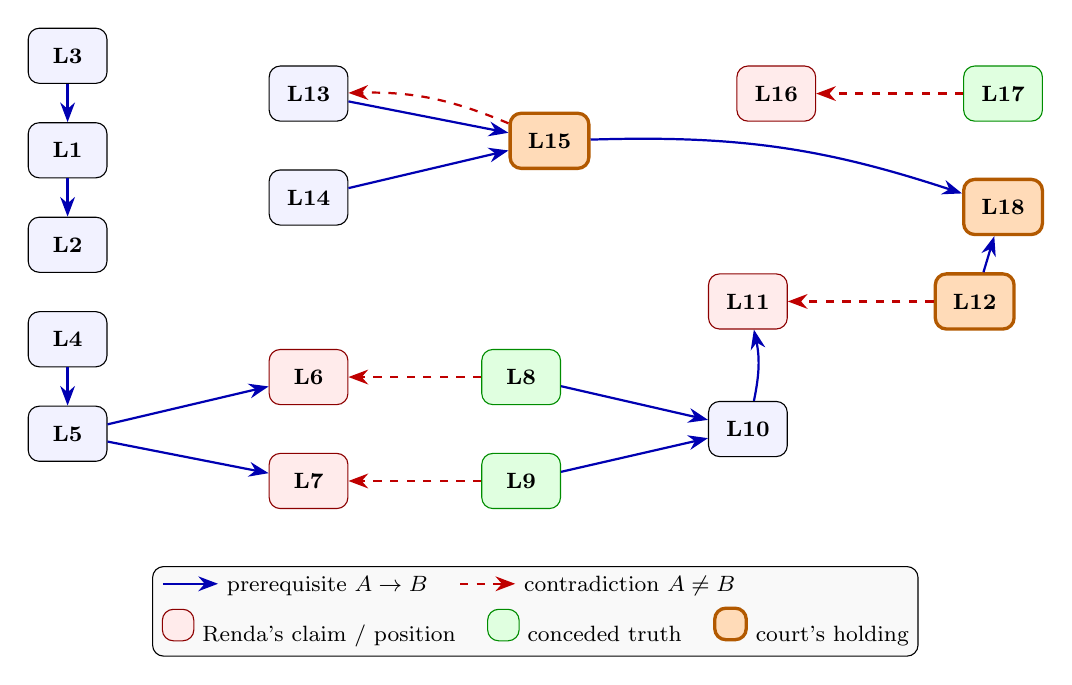
\begin{tikzpicture}[
    >={Stealth[length=2.5mm]},
    x=18mm, y=12mm,
    lnode/.style={draw,rounded corners,minimum width=10mm,minimum height=7mm,
                  inner sep=1pt,font=\footnotesize\bfseries,fill=blue!5},
    claim/.style={lnode,fill=red!8,draw=red!55!black},
    truth/.style={lnode,fill=green!12,draw=green!55!black},
    hold/.style={lnode,fill=orange!28,draw=orange!70!black,very thick},
    prereq/.style={->,blue!70!black,thick},
    invalid/.style={->,red!75!black,dashed,thick},
  ]

  % --- prerequisite spine (left, vertical-ish): incident -> conviction -> appeal
  \node[lnode] (l3) at (0,4)   {L3};
  \node[lnode] (l1) at (0,3)   {L1};
  \node[lnode] (l2) at (0,2)   {L2};
  \node[lnode] (l4) at (0,1)   {L4};
  \node[lnode] (l5) at (0,0)   {L5};

  % --- credibility contradiction pairs (claims left-mid, truths right) ---
  \node[claim] (l6) at (1.7,0.6) {L6};
  \node[claim] (l7) at (1.7,-0.5) {L7};
  \node[truth] (l8) at (3.2,0.6) {L8};
  \node[truth] (l9) at (3.2,-0.5) {L9};
  \node[lnode] (l10) at (4.8,0.05) {L10};

  % --- withdrawal argument pair ---
  \node[claim] (l11) at (4.8,1.4) {L11};
  \node[hold]  (l12) at (6.4,1.4) {L12};

  % --- bad-character cluster (upper right) ---
  \node[lnode] (l13) at (1.7,3.6) {L13};
  \node[lnode] (l14) at (1.7,2.5) {L14};
  \node[hold]  (l15) at (3.4,3.1) {L15};

  % --- counsel reversal pair ---
  \node[claim] (l16) at (5.0,3.6) {L16};
  \node[truth] (l17) at (6.6,3.6) {L17};

  % --- disposition ---
  \node[hold]  (l18) at (6.6,2.4) {L18};

  % --- prerequisite edges ---
  \draw[prereq] (l3) -- (l1);
  \draw[prereq] (l1) -- (l2);
  \draw[prereq] (l4) -- (l5);
  \draw[prereq] (l5) -- (l6);
  \draw[prereq] (l5) -- (l7);
  \draw[prereq] (l8) -- (l10);
  \draw[prereq] (l9) -- (l10);
  \draw[prereq] (l10) to[bend right=12] (l11);
  \draw[prereq] (l13) -- (l15);
  \draw[prereq] (l14) -- (l15);
  % the dismissal L18 follows from the holdings that defeated the challenges
  \draw[prereq] (l12) -- (l18);
  \draw[prereq] (l15) to[bend left=10] (l18);

  % --- contradiction edges ---
  \draw[invalid] (l8) -- (l6);
  \draw[invalid] (l9) -- (l7);
  \draw[invalid] (l12) -- (l11);
  \draw[invalid] (l17) -- (l16);
  \draw[invalid] (l15) to[bend right=12] (l13);

  % --- legend ---
  \node[draw,fill=gray!5,rounded corners,anchor=north,align=left,
        font=\footnotesize] at (3.3,-1.4) {
    \tikz\draw[prereq](0,0)--(7mm,0);~prerequisite $A\rightarrow B$
    \quad
    \tikz\draw[invalid](0,0)--(7mm,0);~contradiction $A\neq B$\\[3pt]
    \tikz\node[claim,minimum width=4mm,minimum height=4mm]{};~Renda's claim / position
    \quad
    \tikz\node[truth,minimum width=4mm,minimum height=4mm]{};~conceded truth
    \quad
    \tikz\node[hold,minimum width=4mm,minimum height=4mm]{};~court's holding
  };

\end{tikzpicture}
\end{center}

\noindent\emph{(For legibility, purely sequential narration links among the
spine atoms L2--L5 and the bracketing of L16/L17 within the contamination
argument are summarised rather than drawn edge-by-edge.)}

\subsection*{A faithful, naturally-ordered summary K}

The summary S above was deliberately ordered (claims first, conceded truths
afterward) to manufacture positional contradictions. For contrast we now give a
\emph{faithful} summary \textbf{K} of the same Renda appeal that follows the
judgment's own logical and chronological order: each disputed claim is reported
\emph{together with} its resolution, and the court's reasoning is presented in
the sequence the court itself adopts. Under this ordering the relation structure
is almost entirely \emph{logical implication}; the only residual tensions are the
two points the court expressly adjudicates, and even these read as holdings that
\emph{resolve} an issue rather than as a later atom flatly contradicting an
earlier one.

\noindent\textbf{Plain text.}
\begin{quote}
Raymond Renda was convicted of attempted robbery before HHJ Van Der Werff and a
jury, and appealed. The charge arose when, at about 2~am on 10~November 2003, he
accosted Robert Flint on Mile End Road, followed him home, and seized him by the
neck while demanding money; because the only real question was whether any
offence had been committed, the trial turned on the relative credibility of Flint
and Renda. Seeking to present himself as a man of positive good character, Renda
testified that his serious head injury had been sustained on duty in the armed
forces and that he was in regular employment as a security guard; in truth,
however, the injury was sustained on holiday in a car accident and the security
work had been only short-term, so that this evidence conveyed a false impression
within s\,105(1). When Renda conceded these matters under cross-examination, the
court held that a concession extracted in cross-examination does not amount to a
withdrawal of the false impression under s\,105(3). To help correct that false
impression, the Crown was permitted to put a July~2001 incident before the jury:
Renda had then been found unfit to plead to assault and given an absolute
discharge, so he was not convicted, yet a jury had found as a fact that he struck
a man from behind with a wooden table leg, and the court held that this act was
reprehensible behaviour within the bad-character provisions notwithstanding the
absence of a conviction. A submission that the resulting evidence was
contaminated under s\,107 was rejected, the court holding that it was not
contaminated, and the appeal was dismissed.
\end{quote}

\noindent\textbf{Annotated.} Each clause is one atomic unit
\textsuperscript{\textbf{\scriptsize K\textit{n}}}. The faithful ordering folds
each disputed claim into its finding, so there are no contradiction colours here:
blue~=~neutral fact, orange~=~court's holding.

\begin{quote}
\fu{cFact}{Raymond Renda was convicted of attempted robbery before HHJ Van Der Werff and a jury, and appealed}{K1}. The charge arose when,
\fu{cFact}{at about 2~am on 10~November 2003, he accosted Robert Flint on Mile End Road, followed him home, and seized him by the neck while demanding money}{K2}; because the only real question was whether any offence had been committed,
\fu{cFact}{the trial turned on the relative credibility of Flint and Renda}{K3}.
\fu{cFact}{Seeking to present himself as a man of positive good character, Renda testified}{K4}
\fu{cFact}{that his serious head injury had been sustained on duty in the armed forces and that he was in regular employment as a security guard}{K5}; in truth, however,
\fu{cFact}{the injury was sustained on holiday in a car accident and the security work had been only short-term, so that this evidence conveyed a false impression within \mbox{s\,105(1)}}{K6}.
\fu{cFact}{When Renda conceded these matters under cross-examination}{K7}, the
\fu{cHold}{court held that a concession extracted in cross-examination does not amount to a withdrawal of the false impression under \mbox{s\,105(3)}}{K8}. To help correct that false impression,
\fu{cFact}{the Crown was permitted to put a July~2001 incident before the jury}{K9}:
\fu{cFact}{Renda had then been found unfit to plead to assault and given an absolute discharge, so he was not convicted}{K10}, yet
\fu{cFact}{a jury had found as a fact that he struck a man from behind with a wooden table leg}{K11}, and the
\fu{cHold}{court held that this act was reprehensible behaviour within the bad-character provisions notwithstanding the absence of a conviction}{K12}.
\fu{cFact}{A submission that the resulting evidence was contaminated under \mbox{s\,107}}{K13} was rejected, the
\fu{cHold}{court holding that it was not contaminated, and the appeal was dismissed}{K14, K15}.
\end{quote}

\subsection*{Atomic units of K (self-contained, in order of appearance)}
\begin{enumerate}[label=\textbf{K\arabic*.},leftmargin=*]
  \item Raymond Renda was convicted of attempted robbery and appealed against the conviction.
  \item Renda accosted Robert Flint on Mile End Road at about 2~am on 10~November 2003, followed him home, and seized him by the neck while demanding money.
  \item The trial turned on the relative credibility of Robert Flint and Raymond Renda.
  \item Renda testified seeking to present himself as a man of positive good character.
  \item Renda testified that his head injury was sustained on duty in the armed forces and that he was in regular employment as a security guard.
  \item In truth Renda's injury was sustained on holiday in a car accident and his security work had been only short-term, so his evidence conveyed a false impression within s\,105(1).
  \item Renda conceded these matters under cross-examination.
  \item The court held that a concession extracted in cross-examination does not amount to a withdrawal of the false impression under s\,105(3).
  \item To help correct the false impression, the Crown was permitted to put a July~2001 incident before the jury.
  \item In the July~2001 incident Renda was found unfit to plead to assault and given an absolute discharge, so he was not convicted.
  \item A jury had found as a fact that Renda struck a man from behind with a wooden table leg.
  \item The court held that the table-leg act was reprehensible behaviour within the bad-character provisions, notwithstanding the absence of a conviction.
  \item A submission was made that the evidence was contaminated under s\,107.
  \item The court held that the evidence was not contaminated.
  \item The appeal was dismissed.
\end{enumerate}

\subsection*{Relations}

\textbf{Logical prerequisites ($A \rightarrow B$).}
\begin{itemize}[leftmargin=*]
  \item K2 $\rightarrow$ K1 --- the attempted-robbery incident grounds the conviction and the appeal.
  \item K1 $\rightarrow$ K3 --- the contested conviction is what makes credibility the trial issue.
  \item K3 $\rightarrow$ K4 --- credibility being decisive is why Renda testified to his good character.
  \item K4 $\rightarrow$ K5 --- the good-character case comprises the specific claims about injury and employment.
  \item K5 $\rightarrow$ K6 --- the claims are what the truth contradicts, yielding the ``false impression'' finding.
  \item K6 $\rightarrow$ K7 --- there must be a false assertion for Renda to concede it under cross-examination.
  \item K7 $\rightarrow$ K8 --- the cross-examination concession is the act the s\,105(3) holding rules upon.
  \item K6 $\rightarrow$ K9 --- the false impression is what the July~2001 material is admitted to correct.
  \item K10,\,K11 $\rightarrow$ K12 --- the unfit-to-plead finding and the found-fact assault ground the ``reprehensible behaviour'' holding.
  \item K9 $\rightarrow$ K13 --- admitting the bad-character material is the premise of the contamination submission.
  \item K13 $\rightarrow$ K14 --- the contamination submission is what the ``not contaminated'' holding answers.
  \item K8,\,K12,\,K14 $\rightarrow$ K15 --- the three holdings against Renda jointly ground the dismissal.
\end{itemize}

\noindent
\textbf{Contradictions / position invalidations ($A \neq B$).} Under the faithful
ordering there are \emph{no} positional invalidations between asserted atoms:
each claim (K5) is reported together with its correction (K6), so the truth does
not appear later as a contradicting atom but as part of the same finding. The two
genuine tensions in the case are stated as \emph{holdings that resolve} an issue,
not as contradictions:
\begin{itemize}[leftmargin=*]
  \item K8 settles the s\,105(3) question (a forced concession is not a withdrawal) --- presented as a ruling, with no competing asserted atom left standing.
  \item K12 settles the reprehensible-behaviour question (conduct can be reprehensible though it produced no conviction, K10) --- again a ruling rather than a flat contradiction.
\end{itemize}

\noindent
\textbf{Note.} Comparing K with S (the same facts, deliberately reordered)
illustrates the point: positional invalidation is a property of how a text is
\emph{arranged}, not only of the facts it contains. A faithful, logically ordered
summary of \emph{Renda} carries the case's full content as an implication chain
from the incident (K2) to the dismissal (K15), with the disputed points absorbed
into the findings rather than surfacing as contradictions.

\subsection*{Relation graph}

Solid blue arrows are logical prerequisites ($A \rightarrow B$). The court's three
operative holdings (K8, K12, K14) are highlighted; together they ground the
dismissal K15. There are no contradiction edges --- the faithful ordering folds
each disputed claim into its finding. Nodes are placed on an explicit grid so no
edge crosses a node.

\begin{center}
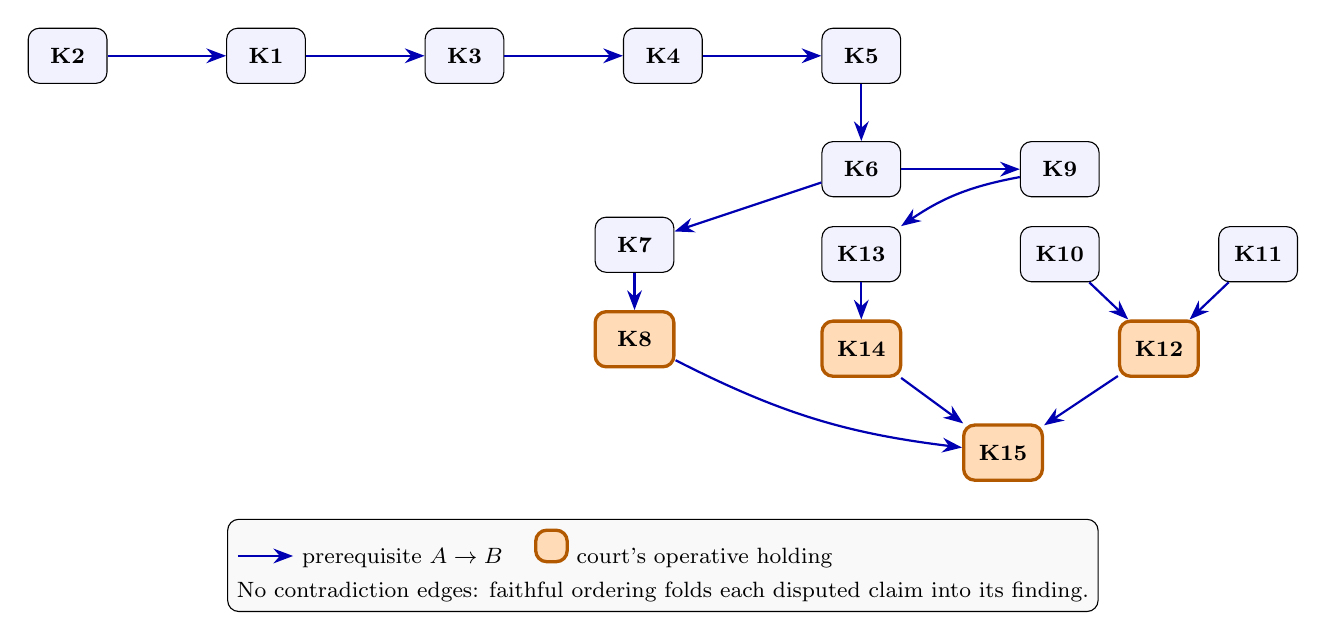
\begin{tikzpicture}[
    >={Stealth[length=2.5mm]},
    x=18mm, y=12mm,
    knode/.style={draw,rounded corners,minimum width=10mm,minimum height=7mm,
                  inner sep=1pt,font=\footnotesize\bfseries,fill=blue!5},
    hold/.style={knode,fill=orange!28,draw=orange!70!black,very thick},
    prereq/.style={->,blue!70!black,thick},
  ]

  % --- main spine (incident -> credibility -> good character -> claims) ---
  \node[knode] (k2) at (0,3)   {K2};
  \node[knode] (k1) at (1.4,3) {K1};
  \node[knode] (k3) at (2.8,3) {K3};
  \node[knode] (k4) at (4.2,3) {K4};
  \node[knode] (k5) at (5.6,3) {K5};

  % --- false impression and its two downstream branches ---
  \node[knode] (k6) at (5.6,1.8) {K6};

  % withdrawal branch (left-down)
  \node[knode] (k7) at (4.0,1.0) {K7};
  \node[hold]  (k8) at (4.0,0.0) {K8};

  % bad-character / correction branch (right-down)
  \node[knode] (k9)  at (7.0,1.8) {K9};
  \node[knode] (k10) at (7.0,0.9) {K10};
  \node[knode] (k11) at (8.4,0.9) {K11};
  \node[hold]  (k12) at (7.7,-0.1) {K12};
  \node[knode] (k13) at (5.6,0.9) {K13};
  \node[hold]  (k14) at (5.6,-0.1) {K14};

  % --- disposition ---
  \node[hold]  (k15) at (6.6,-1.2) {K15};

  % --- prerequisite edges ---
  \draw[prereq] (k2) -- (k1);
  \draw[prereq] (k1) -- (k3);
  \draw[prereq] (k3) -- (k4);
  \draw[prereq] (k4) -- (k5);
  \draw[prereq] (k5) -- (k6);
  \draw[prereq] (k6) -- (k7);
  \draw[prereq] (k7) -- (k8);
  \draw[prereq] (k6) -- (k9);
  \draw[prereq] (k10) -- (k12);
  \draw[prereq] (k11) -- (k12);
  \draw[prereq] (k9) to[bend right=12] (k13);
  \draw[prereq] (k13) -- (k14);
  \draw[prereq] (k8)  to[bend right=10] (k15);
  \draw[prereq] (k12) -- (k15);
  \draw[prereq] (k14) -- (k15);

  % --- legend ---
  \node[draw,fill=gray!5,rounded corners,anchor=north,align=left,
        font=\footnotesize] at (4.2,-1.9) {
    \tikz\draw[prereq](0,0)--(7mm,0);~prerequisite $A\rightarrow B$
    \quad
    \tikz\node[hold,minimum width=4mm,minimum height=4mm]{};~court's operative holding\\[3pt]
    No contradiction edges: faithful ordering folds each disputed claim into its finding.
  };

\end{tikzpicture}
\end{center}

\end{document}
